
%%% Uncomment for slide version
\documentclass[xcolor=dvipsnames]{beamer}
\setbeameroption{hide notes} % Only slides

%%% Uncomment for handout version
%\documentclass[handout]{beamer}
%\setbeameroption{show notes on second screen=right} % Both
\usepackage{indentfirst}

\usepackage{enumitem}
\usepackage{listings}
\usepackage{adjustbox} % To incorporate code into Latex
\usepackage{multirow} % To merge multiple rows  in a table
\usepackage{soul} % To put in strikethrough text
\usepackage{array}
\usepackage{makecell}

\setbeamertemplate{note page}{\pagecolor{white}\insertnote}
\setbeamertemplate{footline}{}
\usetheme[progressbar=frametitle]{moloch}% modern fork of the metropolis theme
\setbeamercolor{background canvas}{bg=white}
\setbeamercolor{frametitle}{fg=black,bg=ProcessBlue!20}

\setbeamercolor{progress bar}{use=palette primary,fg=black,bg=black}
\setbeamercolor{note page}{bg=white} 
\setbeamertemplate{date}{}


\DeclareUnicodeCharacter{0313}{*************************************}

\setbeamertemplate{page number in head/foot}{}


\addtobeamertemplate{navigation symbols}{}{%
	\usebeamerfont{footline}%
	\usebeamercolor[fg]{footline}%
	\hspace{1em}%
	\insertframenumber/\inserttotalframenumber
}
\setbeamercolor{itemize item}{fg=black}
\setbeamercolor{itemize subitem}{fg=black}
\setbeamercolor{itemize subsubitem}{fg=black}

\newcommand\blfootnote[1]{%
	\begingroup
	\renewcommand\thefootnote{}\footnote{#1}%
	\addtocounter{footnote}{-1}%
	\endgroup
}

\setlength{\parindent}{0pt}
\newcommand{\forceindent}{\leavevmode{\parindent=1em\indent}}


%%%%%%%%%%%%%%%%%%
%%%%%%%%%%%%%%%%%%
%%%%%%%%%%%%%%%%%%
%%%%%%%%%%%%%%%%%%
%%%%%%%%%%%%%%%%%%
%%%%%%%%%%%%%%%%%%
%%%%%%%%%%%%%%%%%%




\title{\Huge FRST302: Forest Genetics}
\author{\Large Lecture 4.2 -  Accelerating Tree Improvement II}
\date{\today}

\begin{document}
	\maketitle	
	\begin{frame}
	\frametitle{Recap}
	\begin{itemize}
%		\item There are numerous ways to suvey genetic markers at scale (e.g. WGS, reduced representation sequncing, SNP-chips)
		\item Association genetics is a powerful way to identify genes underlying important traits
		\item Association genetics \textbf{is not} a silver bullet as there are multiple statistical issues
		\item Good at identifying large effect loci
	
	\end{itemize}

\end{frame}


\begin{frame}
	
\frametitle{Now What?}
We identified a locus that increases a carrier's height by 3m!\\
			
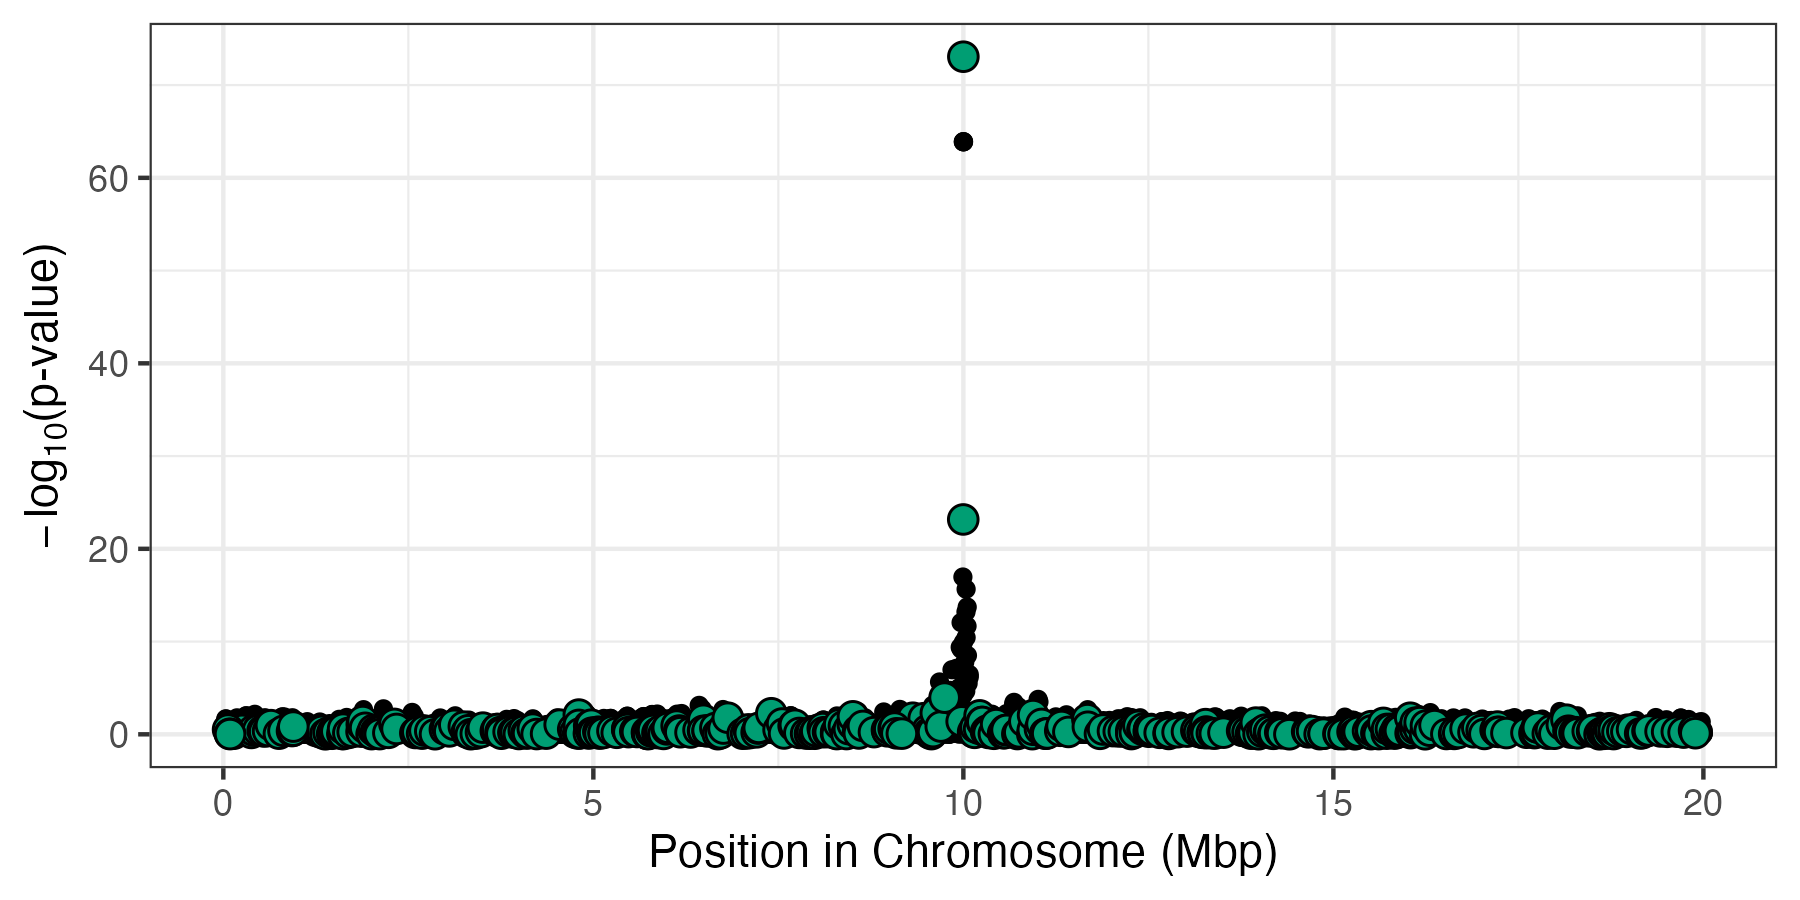
\includegraphics[keepaspectratio, width  = 0.7\textwidth]{img/corPlot_unCorrectedLine.png}


%%%
\begin{columns}
	\begin{column}{0.5\textwidth}
		\centering	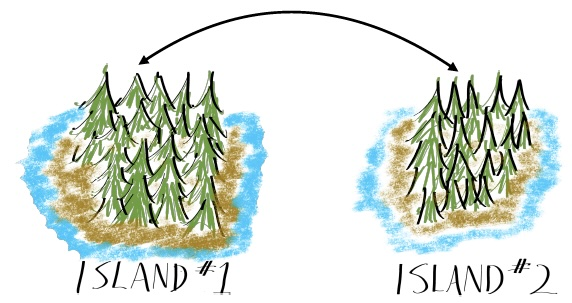
\includegraphics[keepaspectratio, width  = 0.7\textwidth]{img/treeIslands}
	\end{column}
	\begin{column}{0.5\textwidth}
		\begin{itemize}

			\item \textbf{What are we going to do with that information?}
			
		\end{itemize}
	\end{column}
\end{columns}


\end{frame}

\begin{frame}
	\frametitle{Overview for Today}
	\begin{itemize}
		\item[--] Introduction to genetic modification and genome editing
		\item[--] Methods of genetic modification and genome editing
		\item[--] Application of these in forest biology
	\end{itemize}
\end{frame}

\begin{frame}
	\frametitle{Major Milestones in Plant Breeding}
\centering	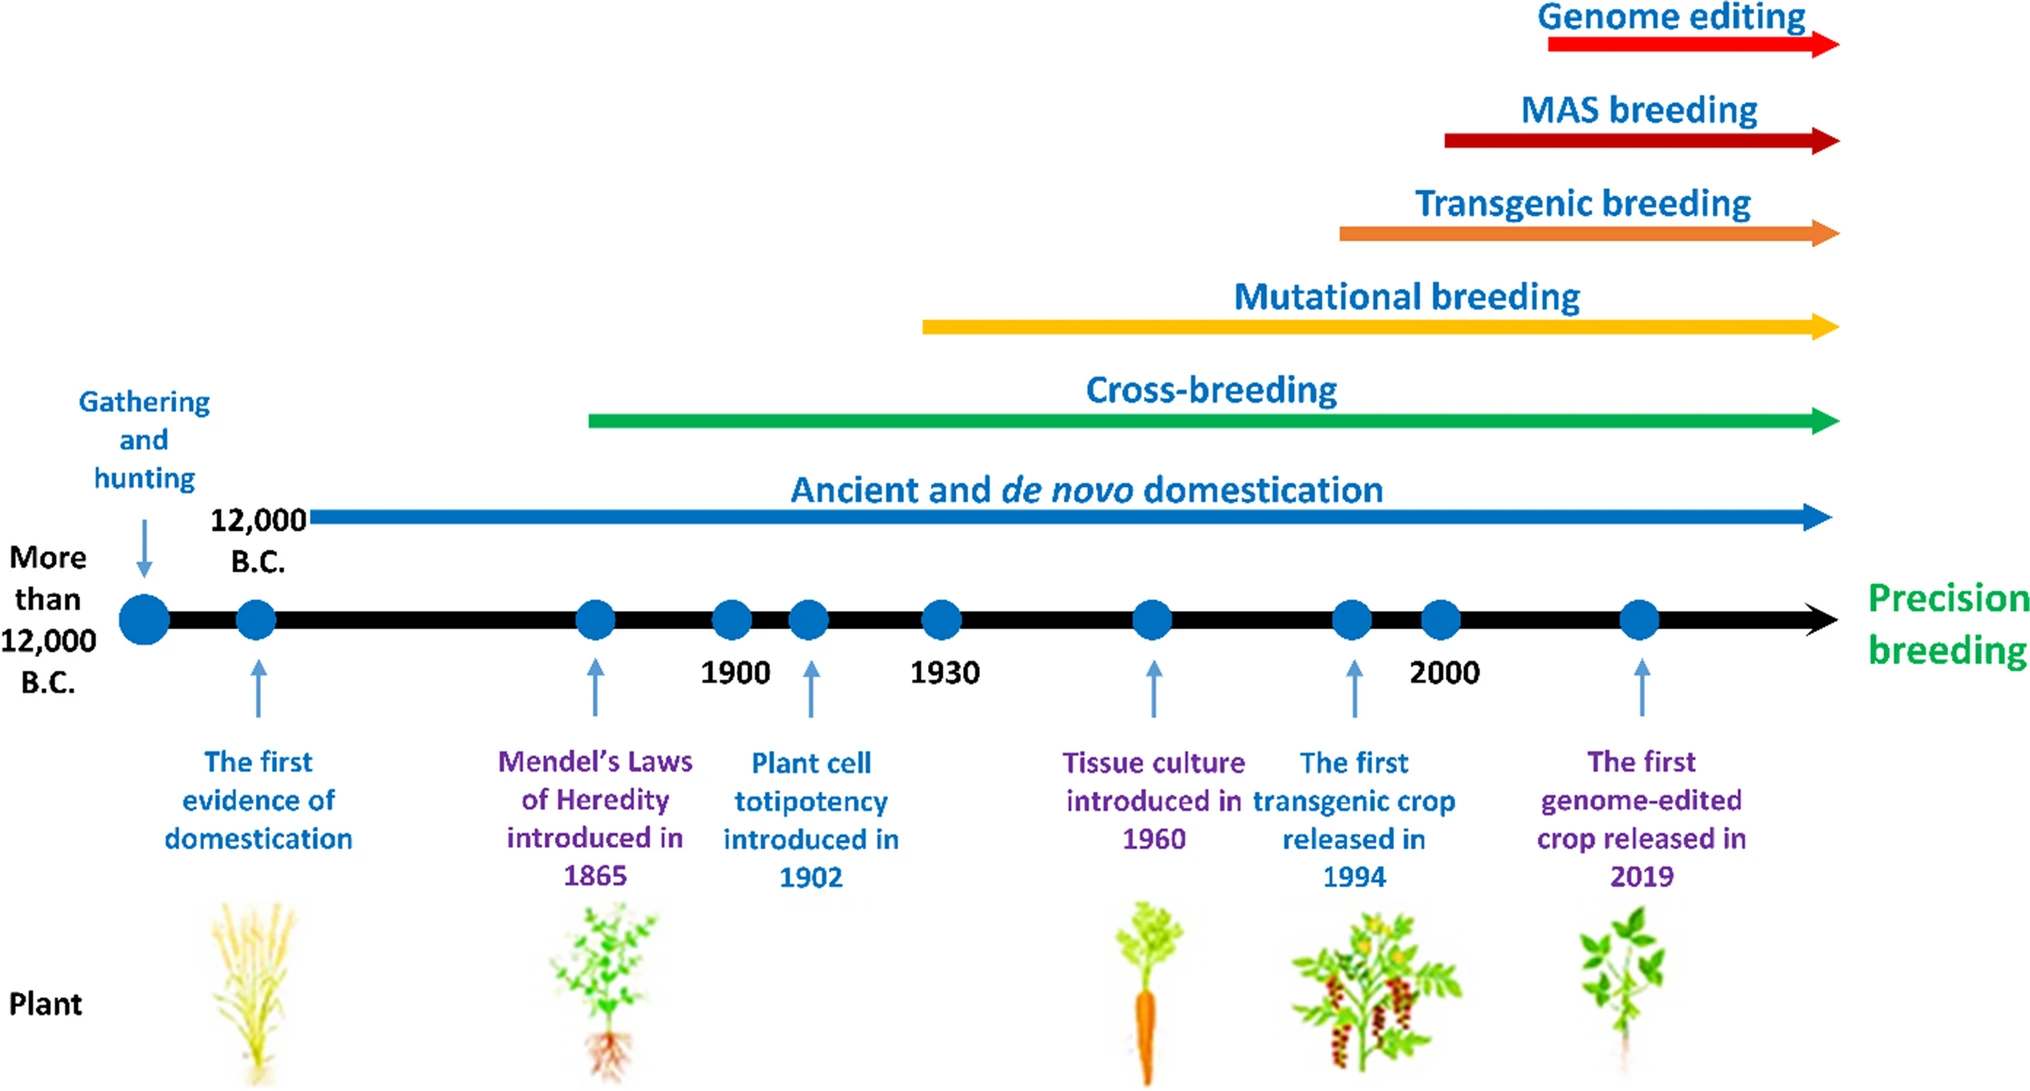
\includegraphics[keepaspectratio, width  = 0.9\textwidth]{img/timeLine}
	
	
	\begin{columns}
		\begin{column}{0.5\textwidth}
		\begin{itemize}
		\item[\textbf{1}] Domestication/traditional breeding
		\item[\textbf{2}] Genetics-informed breeding
		\item[\textbf{3}] Mutational breeding
		\end{itemize}
		\end{column}
		\begin{column}{0.5\textwidth}
		\begin{itemize}
		\item[\textbf{4}] Transgenic breeding
		\item[\textbf{5}] Genomic selection
		\item[\textbf{6}] Genome editing
		\end{itemize}
		\end{column}
	\end{columns}
	
\blfootnote{Figure 1 from Van Vu et al. 2022 \textit{Planta}}
	
	

\end{frame}


\begin{frame}
	\frametitle{1. Domestication/Traditional Breeding}
		
	Humans have conciously (and unconciously) altered the traits of many species of plants and animals for time out of mind\\
	\vspace{10pt}
	Artificial selection alters allele frequencies, leading to populations with a desired pattern of trait variation\\
	
	\centering	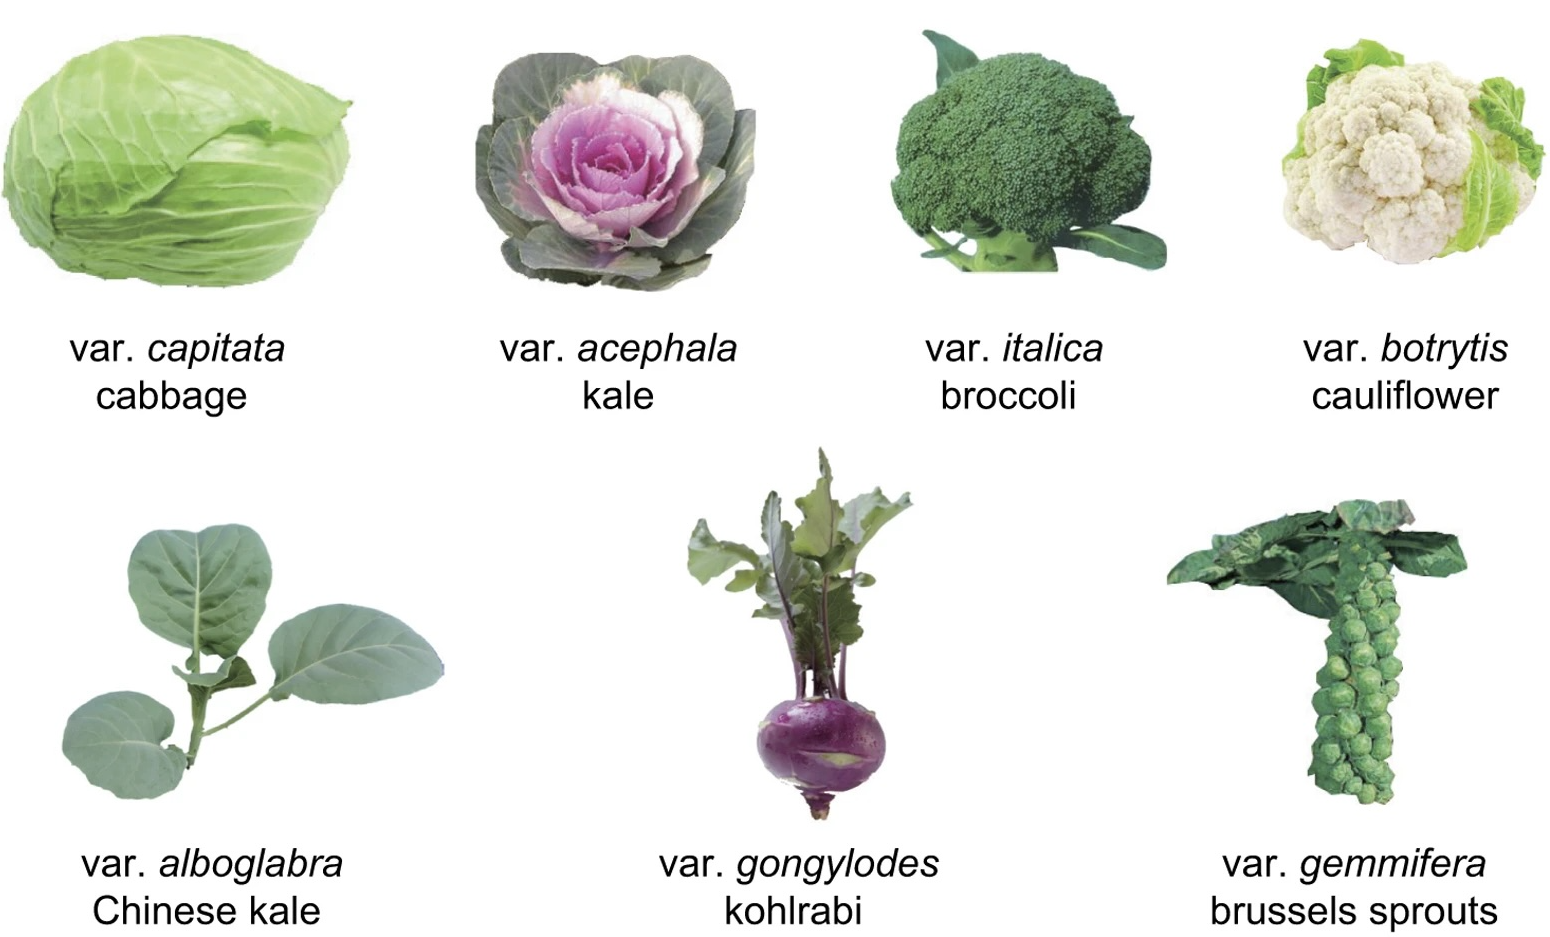
\includegraphics[keepaspectratio, width  = 0.75\textwidth]{img/miniBrassica}
	
	\blfootnote{Modified from Cheng et al 2016 \textit{Scientific Data}}
\end{frame}


\begin{frame}
	\frametitle{Major Milestones in Plant Breeding}
	\centering	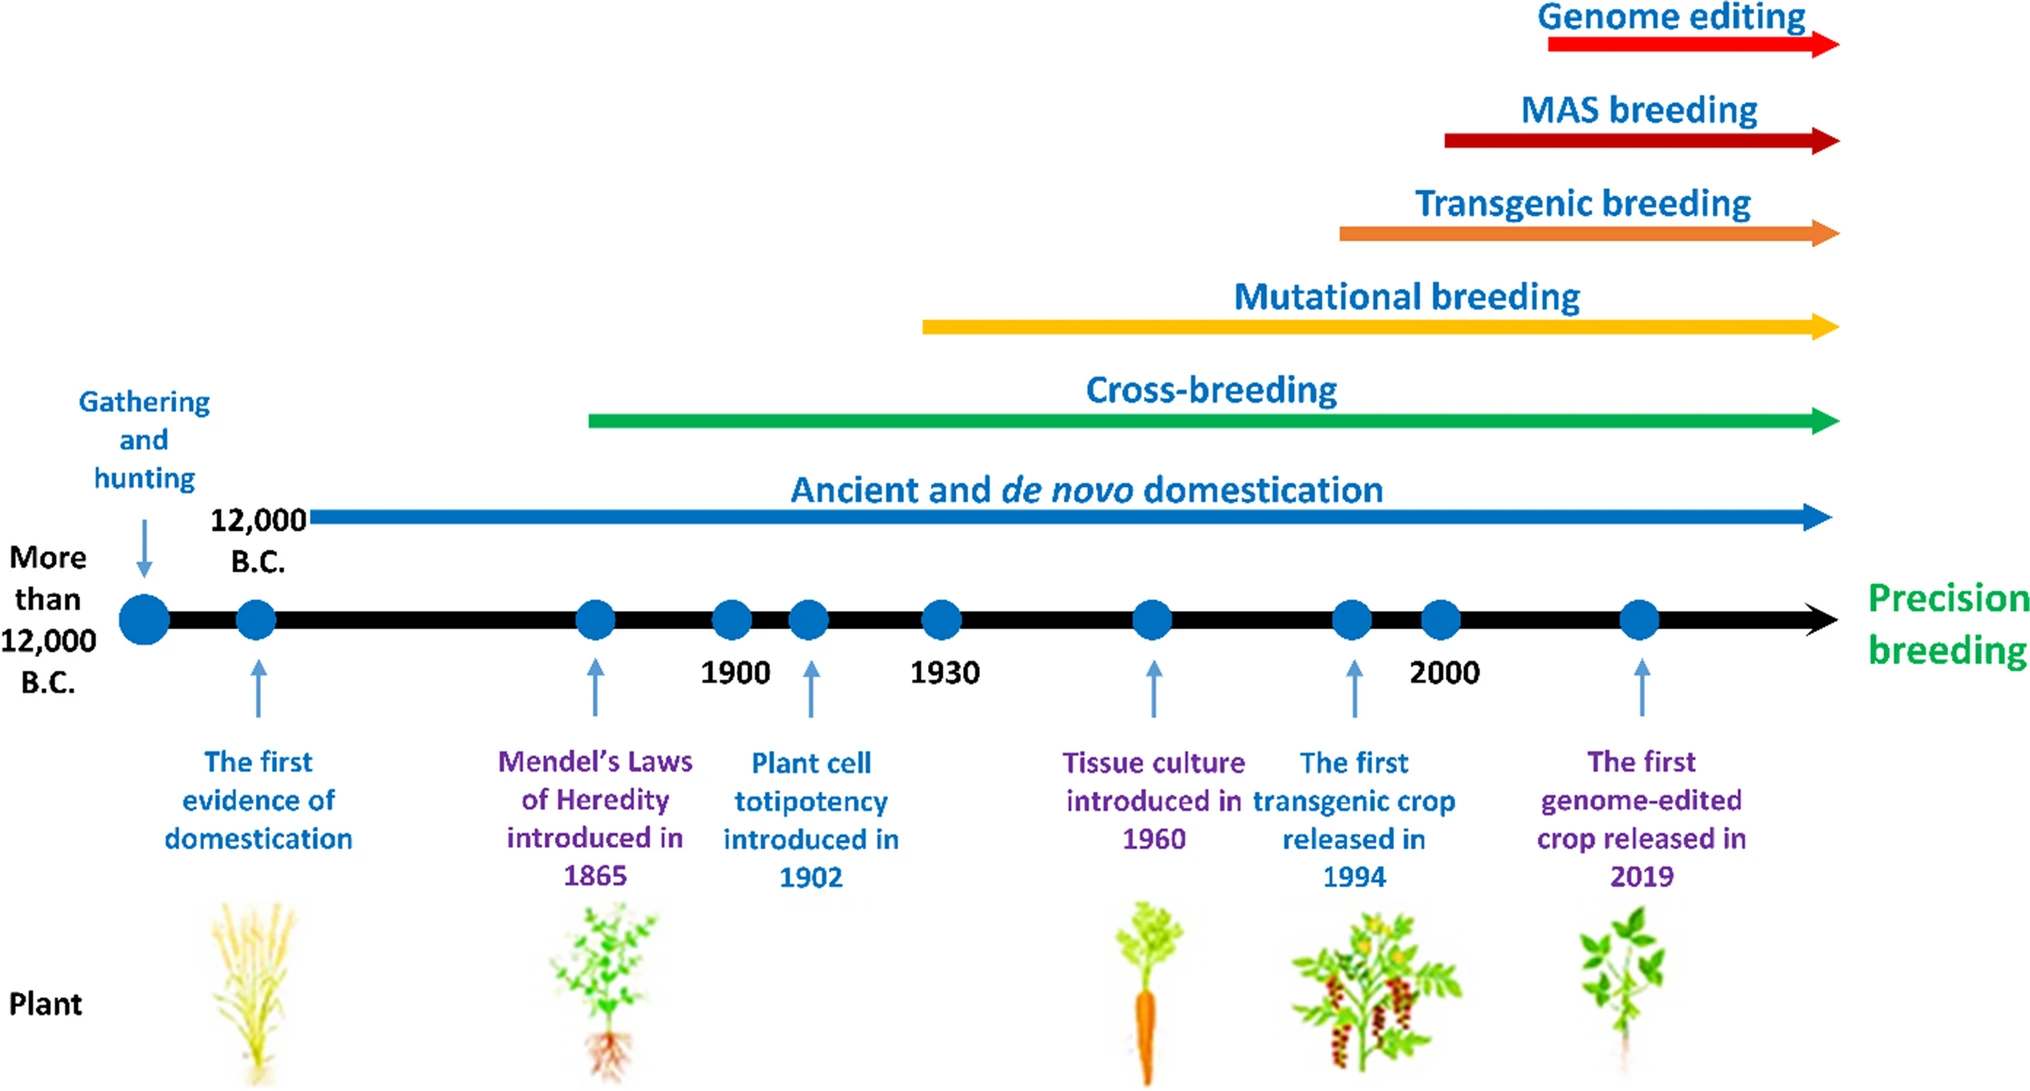
\includegraphics[keepaspectratio, width  = 0.9\textwidth]{img/timeLine}
	
	
	\begin{columns}
		\begin{column}{0.5\textwidth}
			\begin{itemize}
				\item[\textbf{1}] \st{Domestication/traditional breeding}
				\item[\textbf{2}] Genetics-informed breeding
				\item[\textbf{3}] Mutational breeding
			\end{itemize}
		\end{column}
		\begin{column}{0.5\textwidth}
			\begin{itemize}
				\item[\textbf{4}] Transgenic breeding
				\item[\textbf{5}] Genomic selection
				\item[\textbf{6}] Genome editing
			\end{itemize}
		\end{column}
	\end{columns}
	
	\blfootnote{Figure 1 from Van Vu et al. 2022 \textit{Planta}}
	
	
	
\end{frame}


\begin{frame}
\frametitle{2. Genetics-informed breeding}
	\begin{columns}
		\begin{column}{0.4\textwidth}
	\textbf{This is what you learned about in Module 3}\\
	
	Each cycle takes from 20-30 years!\\
	
	\vspace{30pt}
	\textit{We already decided that this takes too long!}
	
	
\end{column}
		\begin{column}{0.65\textwidth}
			\centering 	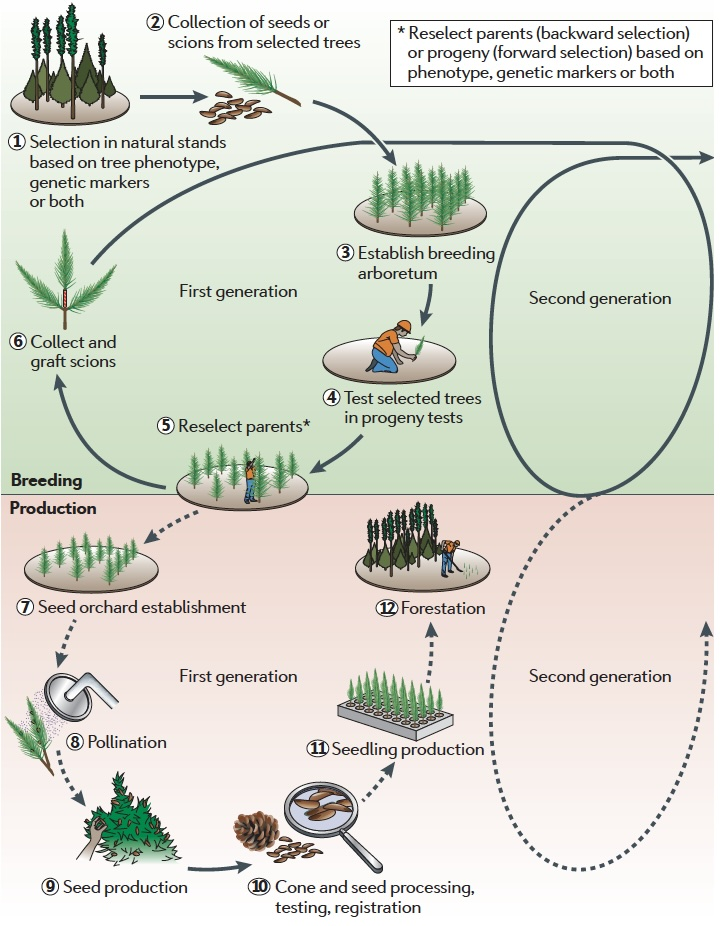
\includegraphics[keepaspectratio, width  = 0.8\textwidth]{img/treeImprovement}
		\end{column}

	\end{columns}
	\blfootnote{Image from Neale and Kremer 2011 \textit{Nature Reviews Genetics}}
\end{frame}




\begin{frame}
	\frametitle{Major Milestones in Plant Breeding}
	\centering	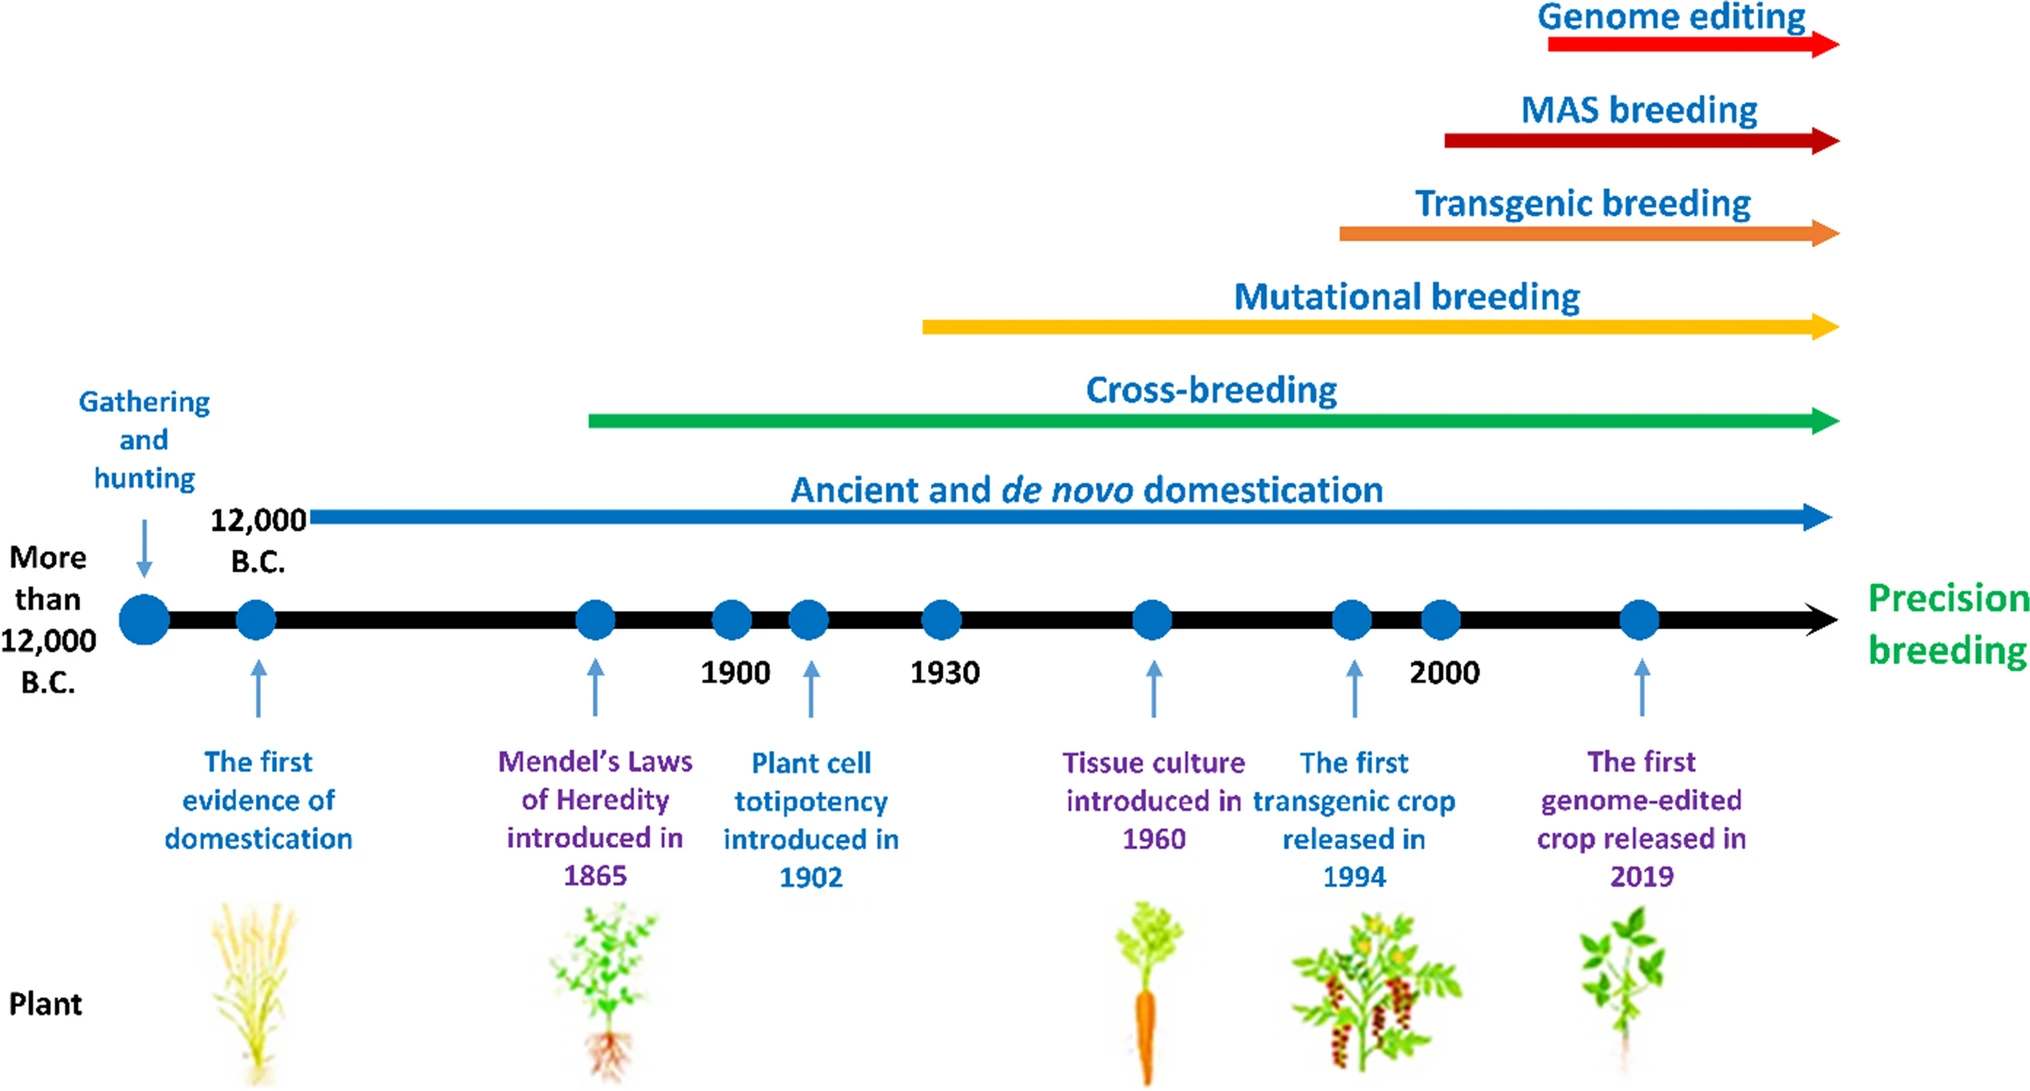
\includegraphics[keepaspectratio, width  = 0.9\textwidth]{img/timeLine}
	
	
	\begin{columns}
		\begin{column}{0.5\textwidth}
			\begin{itemize}
				\item[\textbf{1}] \st{Domestication/traditional breeding}
				\item[\textbf{2}] \st{Genetics-informed breeding}
				\item[\textbf{3}] Mutational breeding
			\end{itemize}
		\end{column}
		\begin{column}{0.5\textwidth}
			\begin{itemize}
				\item[\textbf{4}] Transgenic breeding
				\item[\textbf{5}] Genomic selection
				\item[\textbf{6}] Genome editing
			\end{itemize}
		\end{column}
	\end{columns}
	
	\blfootnote{Figure 1 from Van Vu et al. 2022 \textit{Planta}}
	
	
	
\end{frame}

\begin{frame}
	\frametitle{3. Mutational Breeding}
	Applying mutagenic agents to give rise to desirable traits (e.g. chemicals, X-Rays, even \textit{cosmic} rays!!)
	
	\begin{columns}
		\begin{column}{0.45\textwidth}
						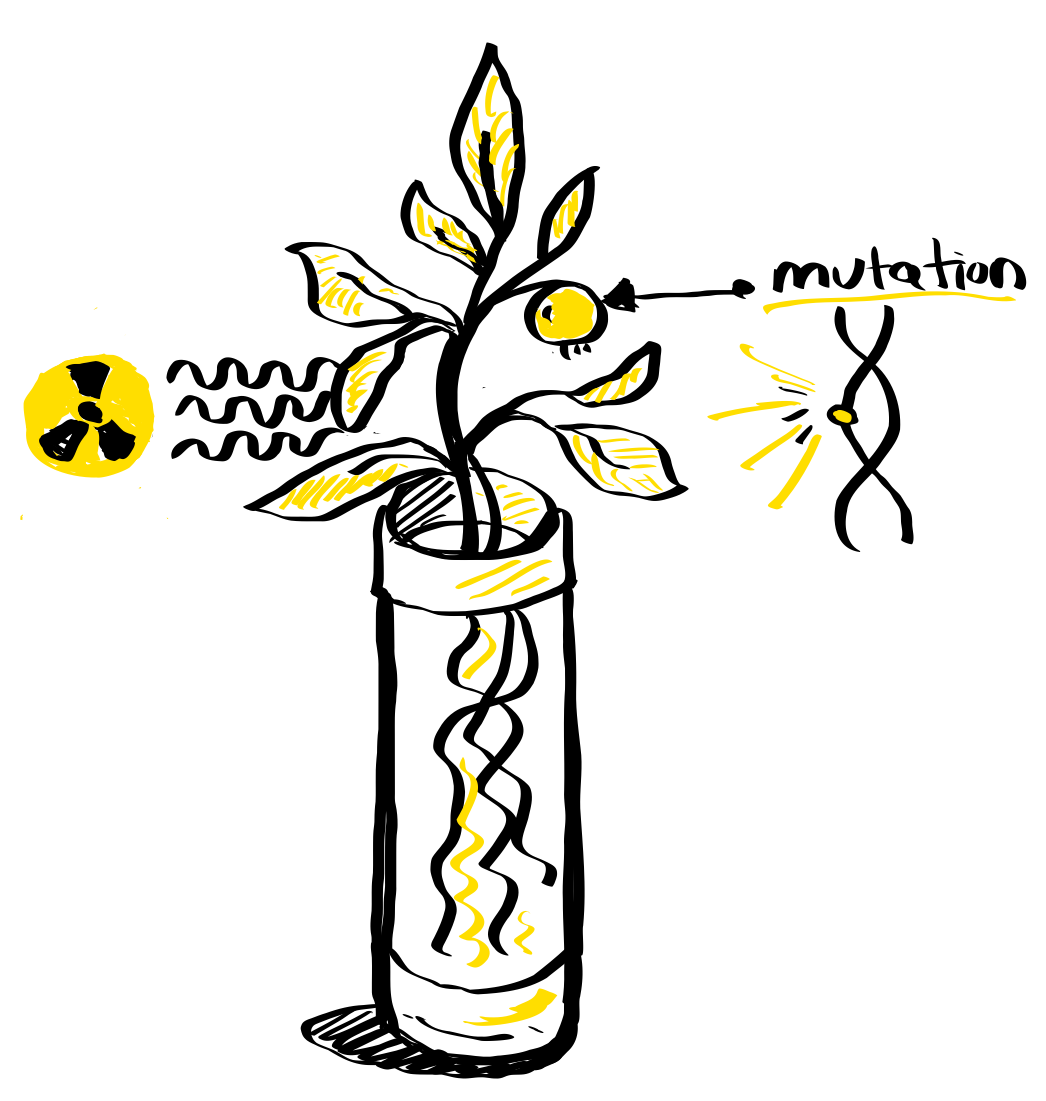
\includegraphics[keepaspectratio, width  = \textwidth]{img/mutationBreeding}	
		\end{column}
		\begin{column}{0.3\textwidth}

\begin{itemize}
	\item[--] Speeds up the natural process of mutation 
	\item[--] Randomly introduces mutation to plant genomes
	\item[--] Widely used in agriculture
\end{itemize}
		\end{column}
		\begin{column}{0.25\textwidth}
			
\includegraphics[keepaspectratio, width  = \textwidth]{img/cosmic}	
				\end{column}
	\end{columns}
	
	
					\blfootnote{L-R; HudsonAlpha Institute, Fantastic Four $\#1$, 1964}
	
\end{frame}


\begin{frame}
	\frametitle{3. Mutational Breeding}
	Applying mutagenic agents to give rise to desirable traits (e.g. chemicals, X-Rays, even \textit{cosmic} rays!!)
	
	\begin{columns}
		\begin{column}{0.45\textwidth}
			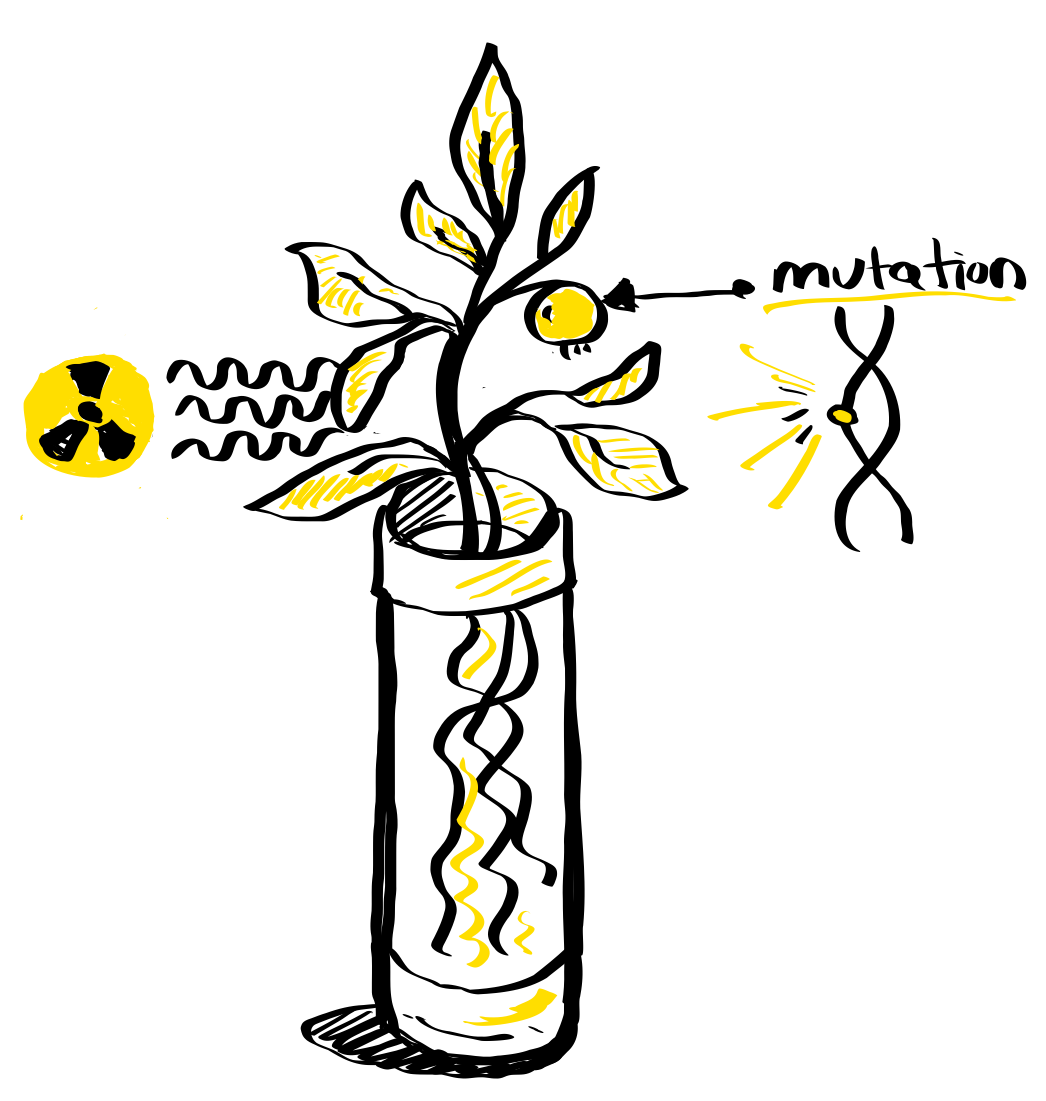
\includegraphics[keepaspectratio, width  = \textwidth]{img/mutationBreeding}	
		\end{column}
		\begin{column}{0.55\textwidth}
		\begin{itemize}
			\item[--] Mutagenesis may give rise to useful mutations	
			\item[--] May lead to harmful ones in addition		
			\item[--] Useful mutants are backcrossed to utilize the new allele
		\end{itemize}			
		\end{column}

		
			\end{columns}
			\textbf{Mutational breeding is not used in forest genetics}
	
	\blfootnote{*\textit{At least as far as I can tell!}}
	\textit{It would be far too slow}
	
\end{frame}




\begin{frame}
	\frametitle{Major Milestones in Plant Breeding}
	\centering	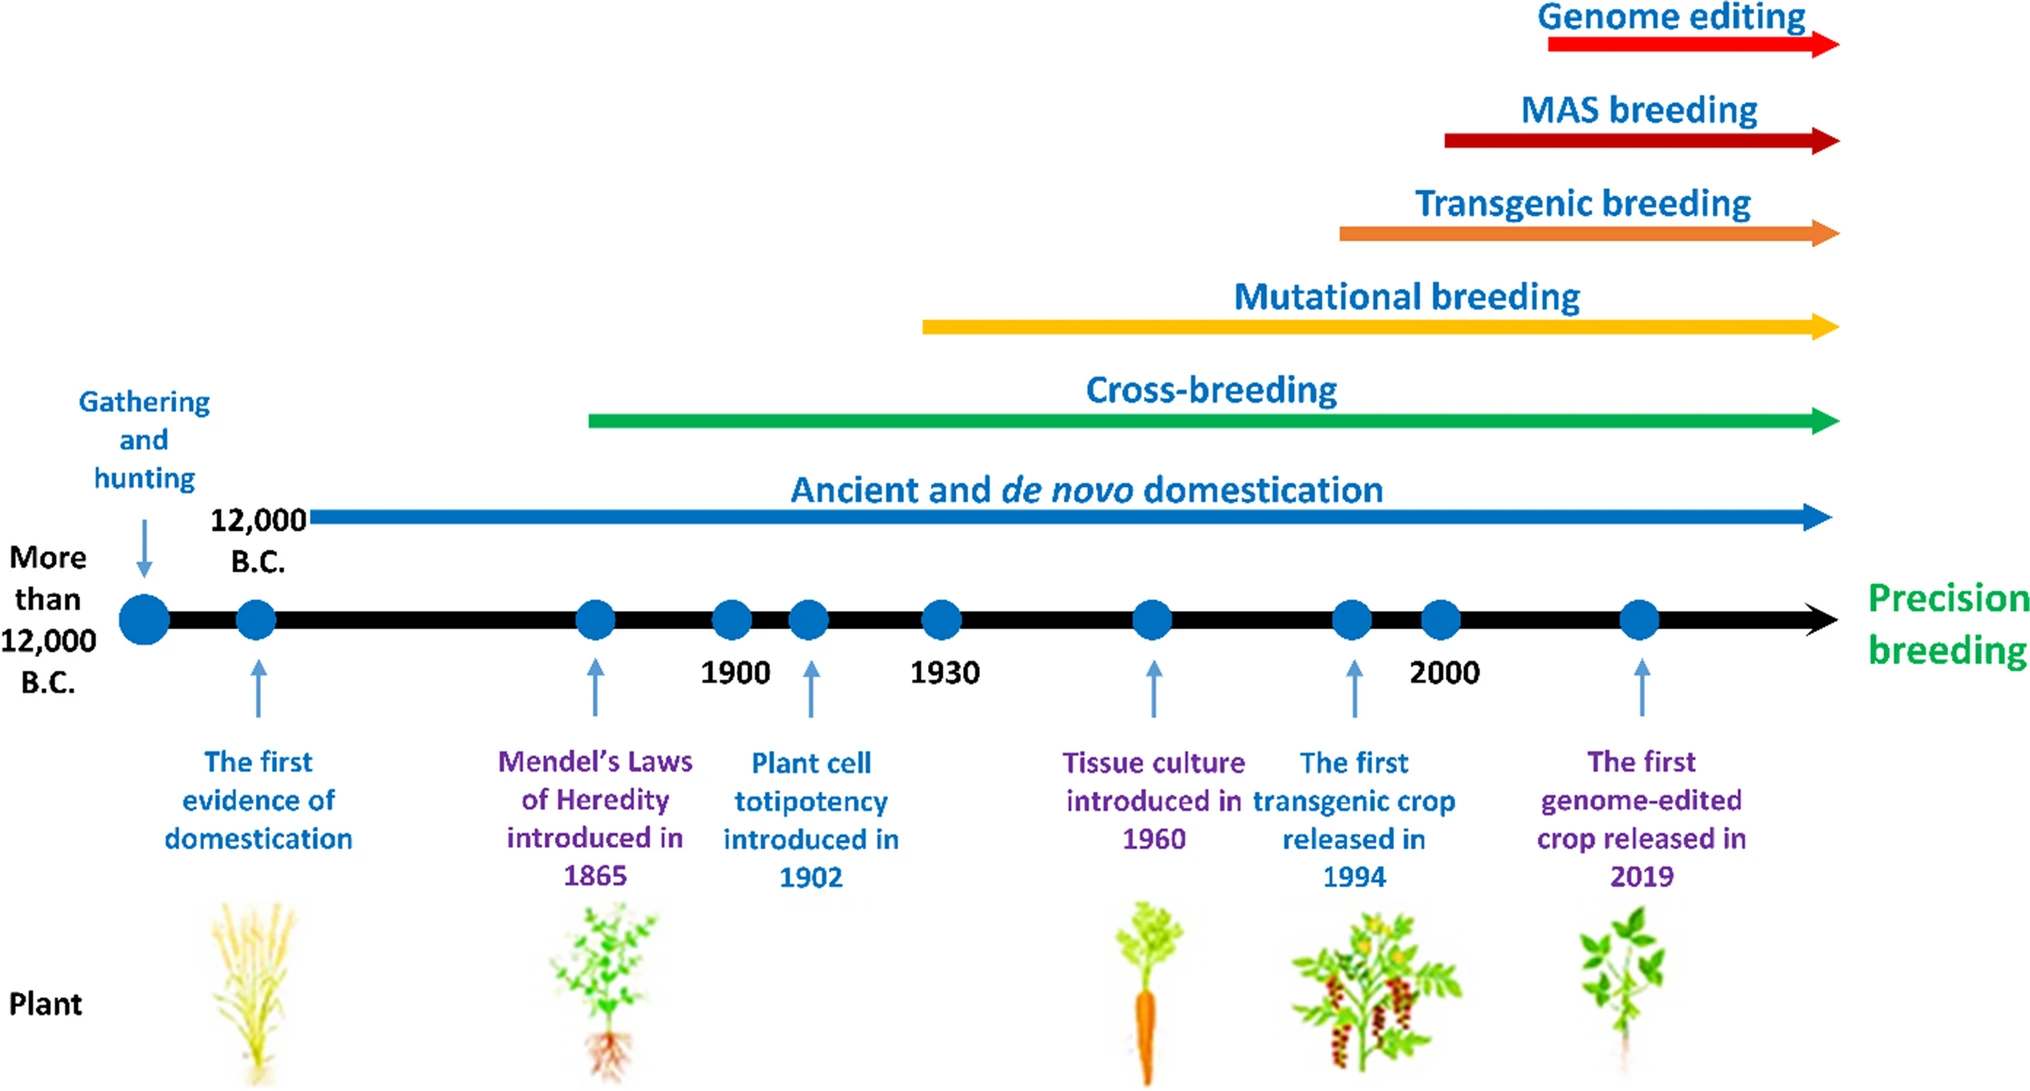
\includegraphics[keepaspectratio, width  = 0.9\textwidth]{img/timeLine}
	
	
	\begin{columns}
		\begin{column}{0.5\textwidth}
			\begin{itemize}
				\item[\textbf{1}] \st{Domestication/traditional breeding}
				\item[\textbf{2}] \st{Genetics-informed breeding}
				\item[\textbf{3}] \st{Mutational breeding}
			\end{itemize}
		\end{column}
		\begin{column}{0.5\textwidth}
			\begin{itemize}
				\item[\textbf{4}] Transgenic breeding
				\item[\textbf{5}] Genomic selection
				\item[\textbf{6}] Genome editing
			\end{itemize}
		\end{column}
	\end{columns}
	
	\blfootnote{Figure 1 from Van Vu et al. 2022 \textit{Planta}}
	
	
	
\end{frame}


\begin{frame}
	\frametitle{4. Transgenic Plant Breeding }
	\textbf{Transgenesis}: using genetic engineering techniques to introduce genes from other lineages, species (or even kingdoms!)\\
	\vspace{20pt}
	
		\centering	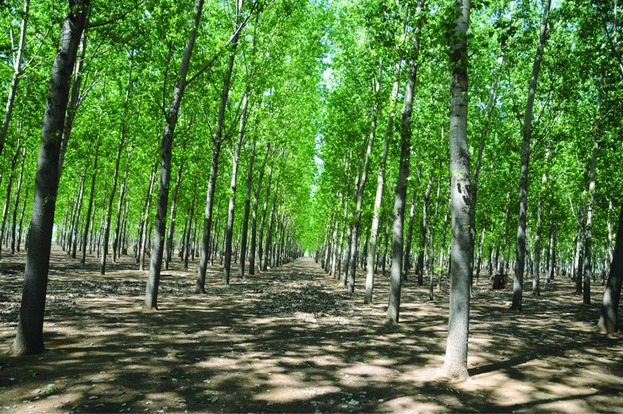
\includegraphics[keepaspectratio, width  = 0.7\textwidth]{img/transgenicPoplar}
	
\blfootnote{Transgenic poplar plantation; Figure 2  Häggman et al 2013 \textit{Plant Biotech}}

	


\end{frame}




\begin{frame}
	\frametitle{4. Transgenic Plant Breeding }
	\begin{columns}
		\begin{column}{0.5\textwidth}
	Genetically Modified Organisms (GMOs) have been a hot topic for many years
	\begin{itemize}
		\item[--] Food safety concerns 
		\item[--] Ethical concerns
		\item[--] Ecological concerns
	\end{itemize}
	
		\end{column}
		\begin{column}{0.5\textwidth}
	\centering	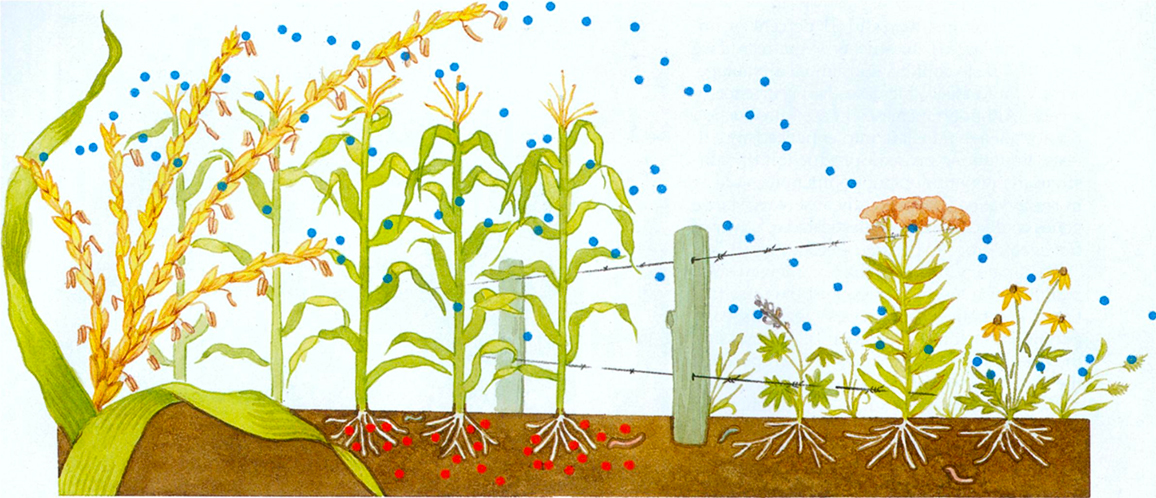
\includegraphics[keepaspectratio, width  = \textwidth]{img/transgenicPollenFlow}
		\end{column}
	\end{columns}
	
	\vspace{10pt}
	The definition of a GMO is still not clear to many people
	
\textit{		E.g., does cloning and selective breeding lead to GMOs?
}
\blfootnote{Image from American Scientist 2001}
\end{frame}
%
\includegraphics[keepaspectratio, width  = 0.7\textwidth]{img/roundUpReady}

\begin{frame}
	\frametitle{What is Genetic Modification?}
	\textbf{Genetic modification (GM)}, or genetic engineering, is the direct manipulation of a organism's genome using biotechnology. \\
	\vspace{10pt}
	\begin{columns}
		\begin{column}{0.45\textwidth}
	
\vspace{10pt}
GM includes:

\begin{itemize}
\item \textbf{Transferring genes} within and across species
\item \textbf{Adding new genes} 
\item \textbf{Knocking out genes} 
\end{itemize}
\vspace{15pt}


\end{column}
\begin{column}{0.55\textwidth}
		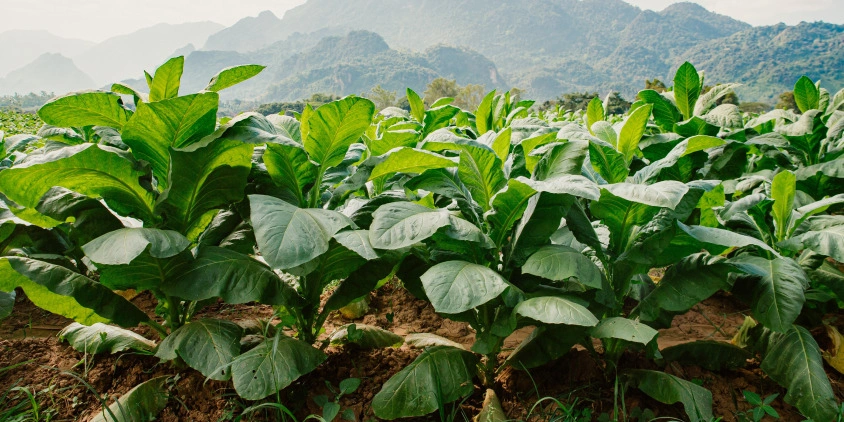
\includegraphics[keepaspectratio, width  = \textwidth]{img/tobacco}		
\end{column}
\end{columns}

The world's first GM plant was produced in 1983\\

\forceindent A gene from the bacterium \textit{Agrobacterium tumefaciens} encoding an anitmicrobial resistance protein was transferred to tobacco


	
\end{frame}


\begin{frame}
	\frametitle{How is GM Acheived in Plants?}
	There are several GM methods that are used in plants:\\
	
	\vspace{15pt}
	\hspace{35pt} \large \textit{Agrobacterium tumefaciens}
	\vspace{5pt}
	\centering
	\begin{columns}
		\begin{column}{0.3\textwidth}
					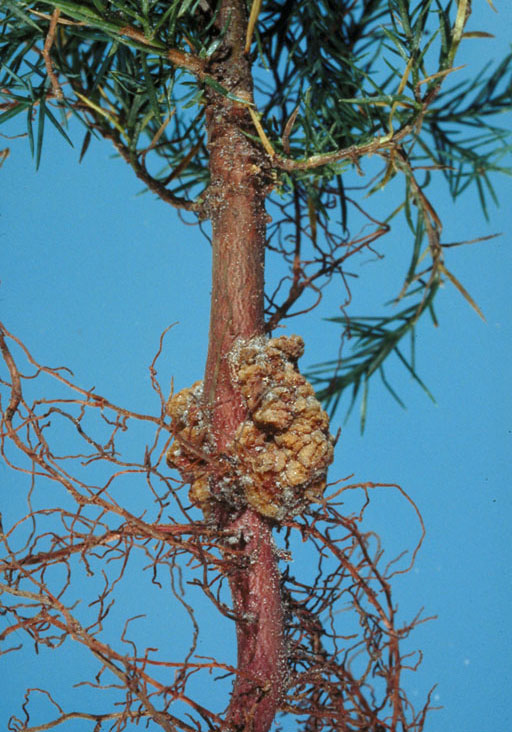
\includegraphics[keepaspectratio, width  = \textwidth]{img/crownGall}		
		\end{column}
		\begin{column}{0.8\textwidth}
			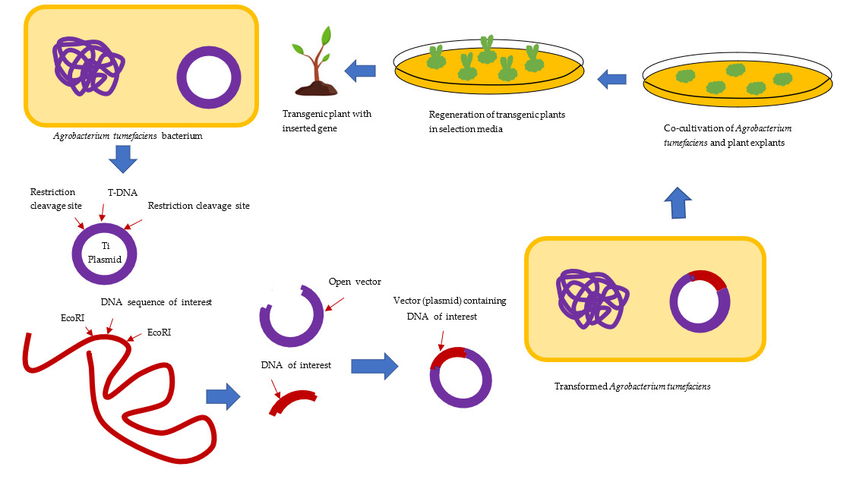
\includegraphics[keepaspectratio, width  = \textwidth]{img/agrobacterium}		
		\end{column}
	\end{columns}	
		\blfootnote{L-R: A crown gall caused by \textit{A. tumefaciens}; Schematic from Ghimire et al. 2023 \textit{Sustainability}}
\end{frame}



\begin{frame}
	\frametitle{How is GM Acheived in Plants?}
	There are several GM methods that are used in plants:\\
	
	\vspace{15pt}
	\hspace{35pt} \large \textit{Gene Gun (a.k.a. BioListics)}
	\vspace{5pt}
	\centering
	\begin{columns}
		\begin{column}{0.3\textwidth}
			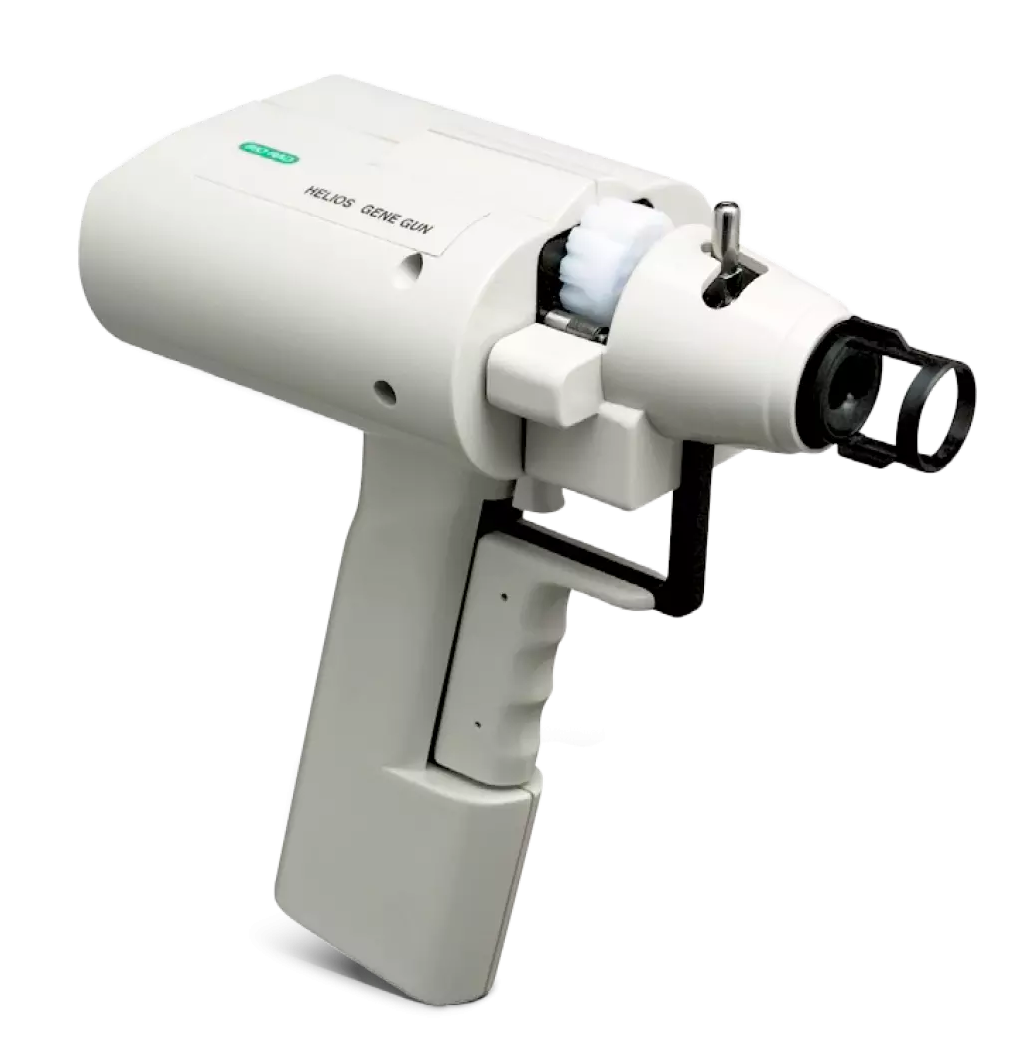
\includegraphics[keepaspectratio, width  = \textwidth]{img/realGeneGun}		
		\end{column}
		\begin{column}{0.8\textwidth}
			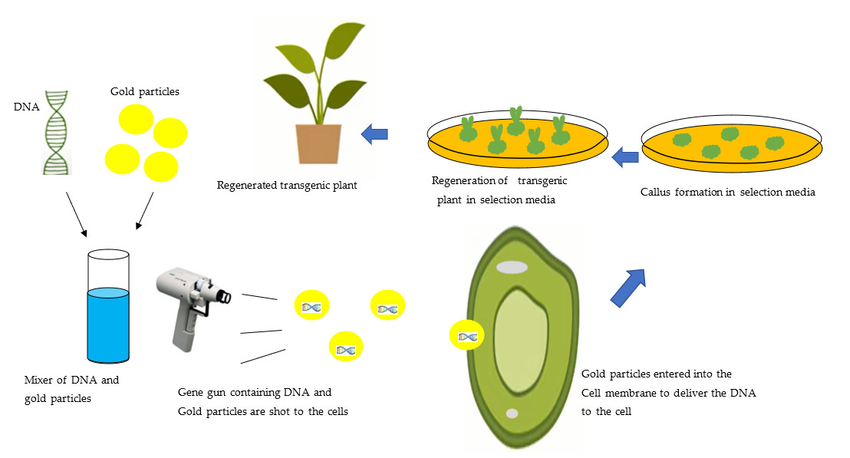
\includegraphics[keepaspectratio, width  = \textwidth]{img/geneGun}		
		\end{column}
	\end{columns}	
	\blfootnote{L-R: Helios GeneGun; Schematic from Ghimire et al. 2023 \textit{Sustainability}}
\end{frame}





\begin{frame}

\scriptsize{Put ethical, ecological and economic concerns aside for the moment...}

\Huge{What are some ways that GM could be used in forest trees?}
	
\end{frame}


\begin{frame}
	\frametitle{Carbon Sequestration}
\centering 	
	Carbon capture and sequestration by growing trees is a so-called "nature-based climate solution"\\
	
\textit{A core component of the carbon economy}\\
	
\vspace{10pt}

\includegraphics[keepaspectratio, width  = 0.7\textwidth]{img/sequestration}\\

\vspace{10pt}
	Engineering trees to better capture and store $CO_2$ seems like a good goal 
	\blfootnote{There is a \textit{LOT} more that could be said about this topic}
\end{frame}



\begin{frame}
	\frametitle{GM in Forest Trees: Example}
	
	Living Carbon is a company based in California that creates ``\textit{bespoke carbon sequestration solutions}"  \\
	\vspace{25pt}
	\begin{columns}
		\begin{column}{0.4\textwidth}
				\centering	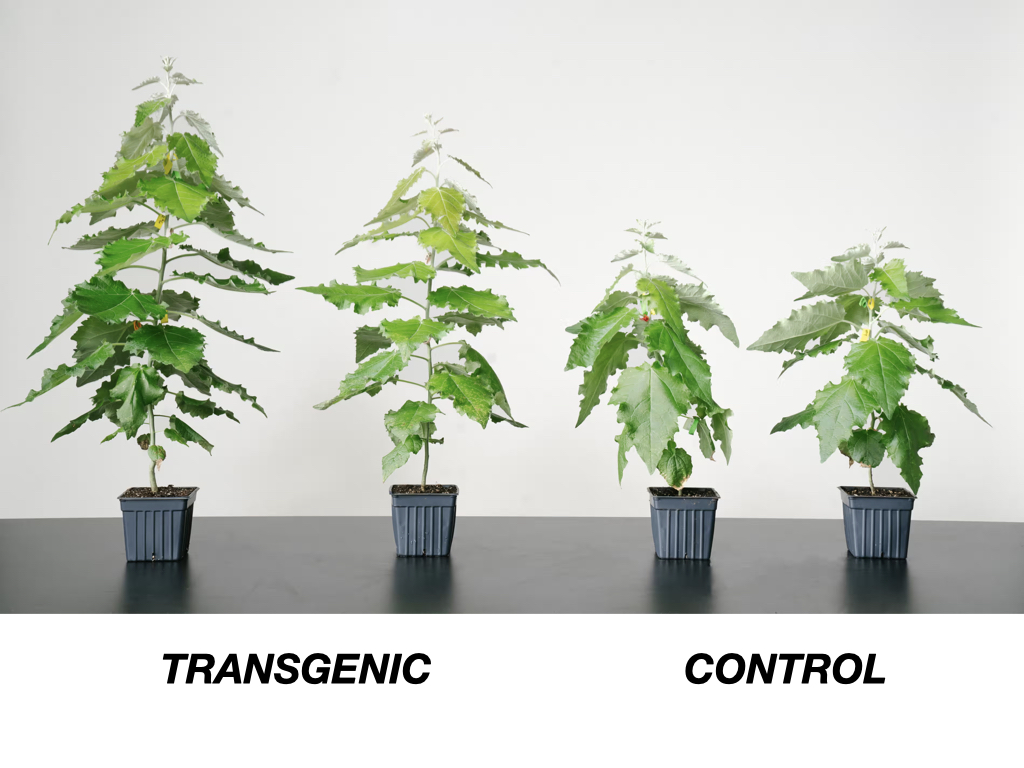
\includegraphics[keepaspectratio, width  = \textwidth]{img/livingCarbon}
		\end{column}
		\begin{column}{0.5\textwidth}
			
			Living Carbon has used GM to develop trees to more efficiently capture carbon
			
		\end{column}
	\end{columns}
\blfootnote{\url{https://www.theguardian.com/environment/2023/oct/15/superpower-plants-absorb-carbon-co2-climate-crisis}}
	
\end{frame}

\begin{frame}
	\frametitle{GM in Forest Trees: Example}
	
	
	\begin{columns}
		\begin{column}{0.5\textwidth}
			\begin{itemize}
				\item[--] In plant cells, chloroplasts carry out photosynthesis
				\item[--] The enzyme at the heart of photosynthesis can also carry out photorespiration to recycle toxic by-products of photosynthesis
				\item[--] \textbf{Photorespiration can reduce the efficiency of the conversion of light into biomass by 20-50\%} 
			\end{itemize}
		\end{column}
		\begin{column}{0.5\textwidth}
						\centering	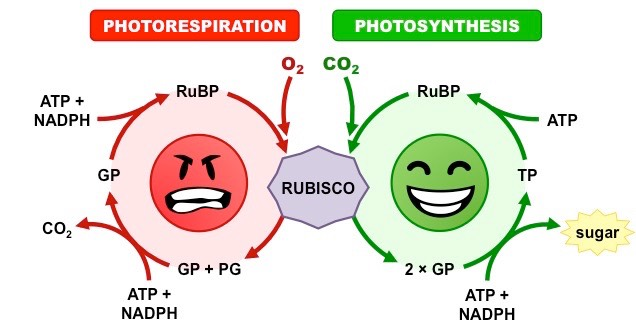
\includegraphics[keepaspectratio, width  = \textwidth]{img/photorespiration}
						\vspace{15pt}

		\end{column}
	\end{columns}
\blfootnote{Don't memorize the molecules; Picture from BioNinja}
	
\end{frame}



\begin{frame}
	\frametitle{GM in Forest Trees: Example}
	
	Living Carbon has produced transgenic hybrid poplar (\textit{Populus tremula × Populus alba})  \\
	

	
	\begin{columns}
		\begin{column}{0.4\textwidth}
			\centering	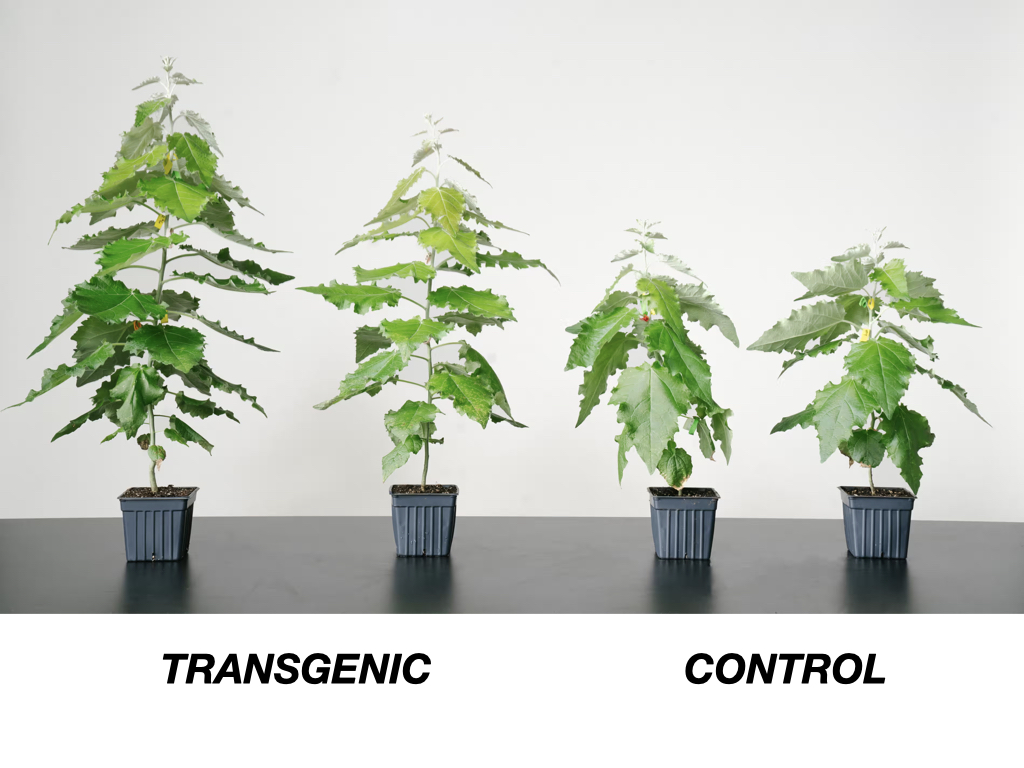
\includegraphics[keepaspectratio, width  = 0.8\textwidth]{img/livingCarbon}\\
						\centering	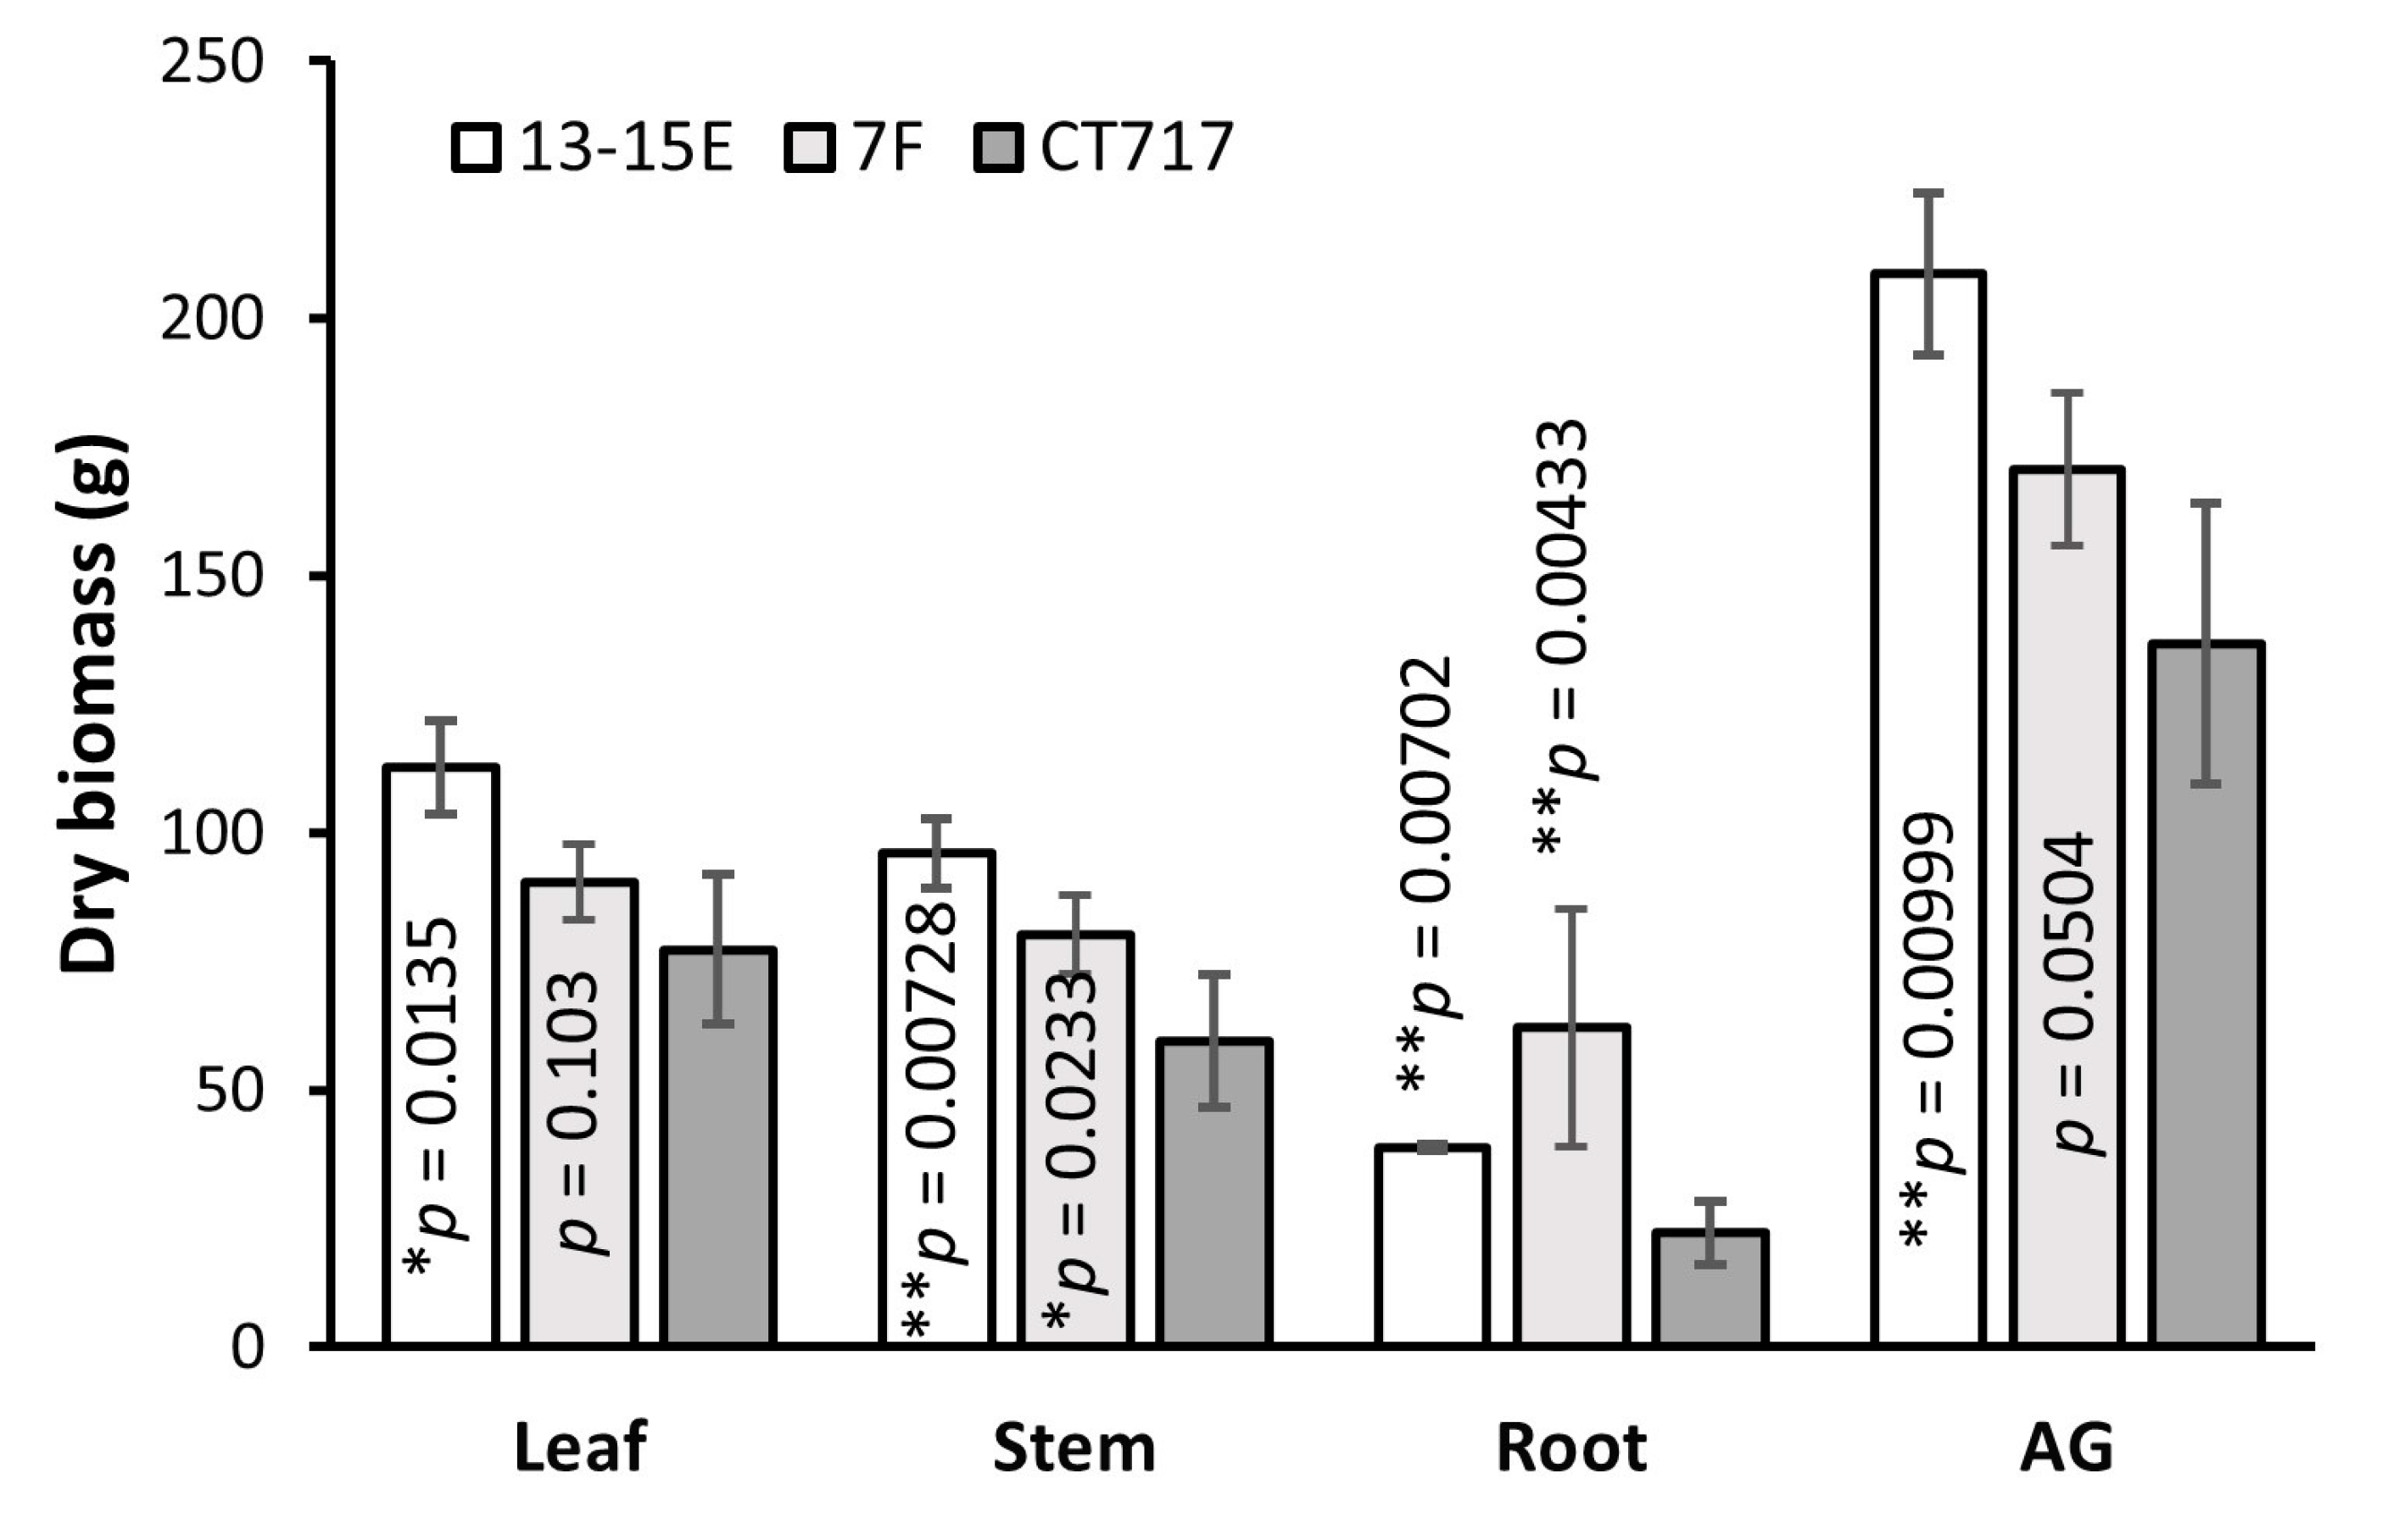
\includegraphics[keepaspectratio, width  = \textwidth]{img/livingCarbonResult}
		\end{column}
		\begin{column}{0.5\textwidth}
			\begin{itemize}
				\item[--] Introduced a gene encoding a small interfering RNA
				\item[--] Silencing a gene involved in photorespiration
				\item[--] Transgenic plants accumulated  up to 53\% more above-ground biomass than controls
				\item[--] Results varied by transgenic line
			\end{itemize}			
		\end{column}
	\end{columns}
	\blfootnote{Tao et al 2023 \textit{Forests}}
	
\end{frame}


\begin{frame}
	\frametitle{Limitations of GM}
	%%%
	\begin{columns}
		\begin{column}{0.5\textwidth}
			\begin{itemize}
				\item[--] The insertion of a new gene may not occur
				\item[--] No control on targeting DNA locations 
				
				
			\end{itemize}
		\end{column}
		\begin{column}{0.5\textwidth}
			\begin{itemize}
				\item[--] One gene at a time
				\item[--] Expensive and slow
				\item[--] Under strict regulation
			\end{itemize}
			
		\end{column}
	\end{columns}
	\vspace{15pt}
	\centering	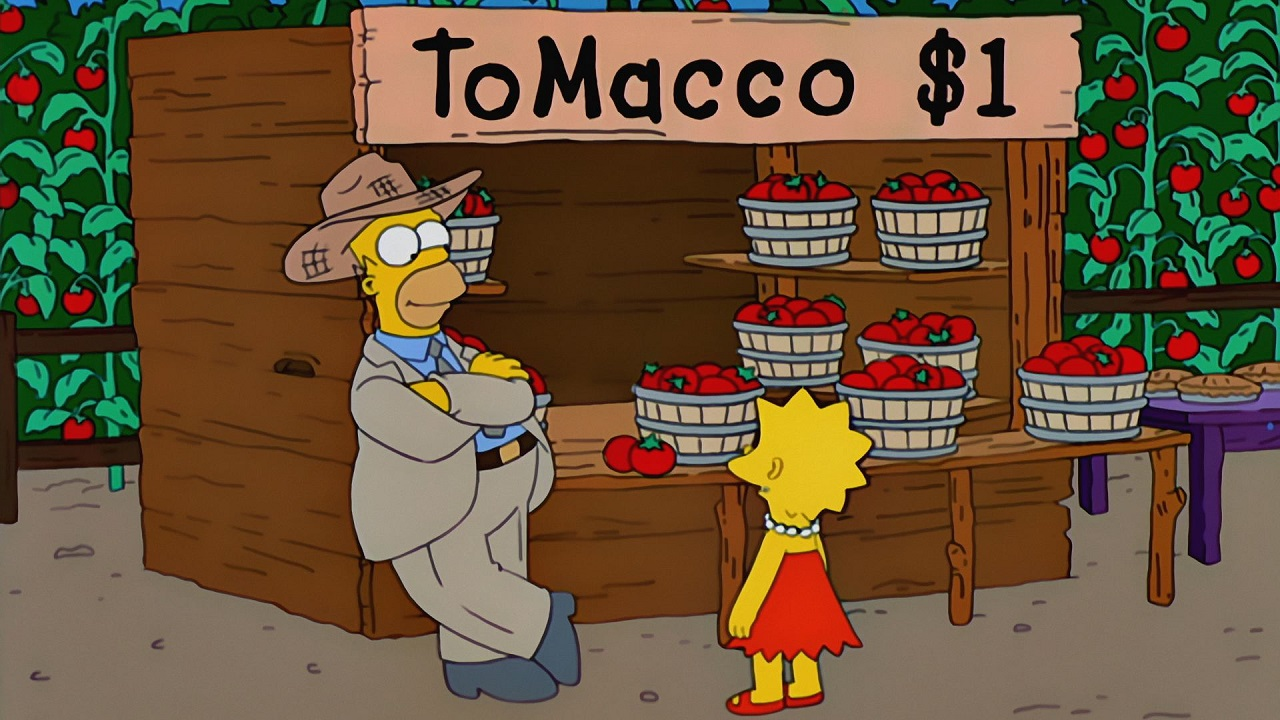
\includegraphics[keepaspectratio, width  = 0.7\textwidth]{img/tomacco}
	\blfootnote{Homer introduced tobacco genes into tomato with a radiation-based procedure to produce his ToMacco}
	
\end{frame}


\begin{frame}
	
	\Huge
	Questions? \\ 
	
\end{frame}

\begin{frame}
	
			\centering	
			Jennifer Doudna and Emmanuelle Charpentier
			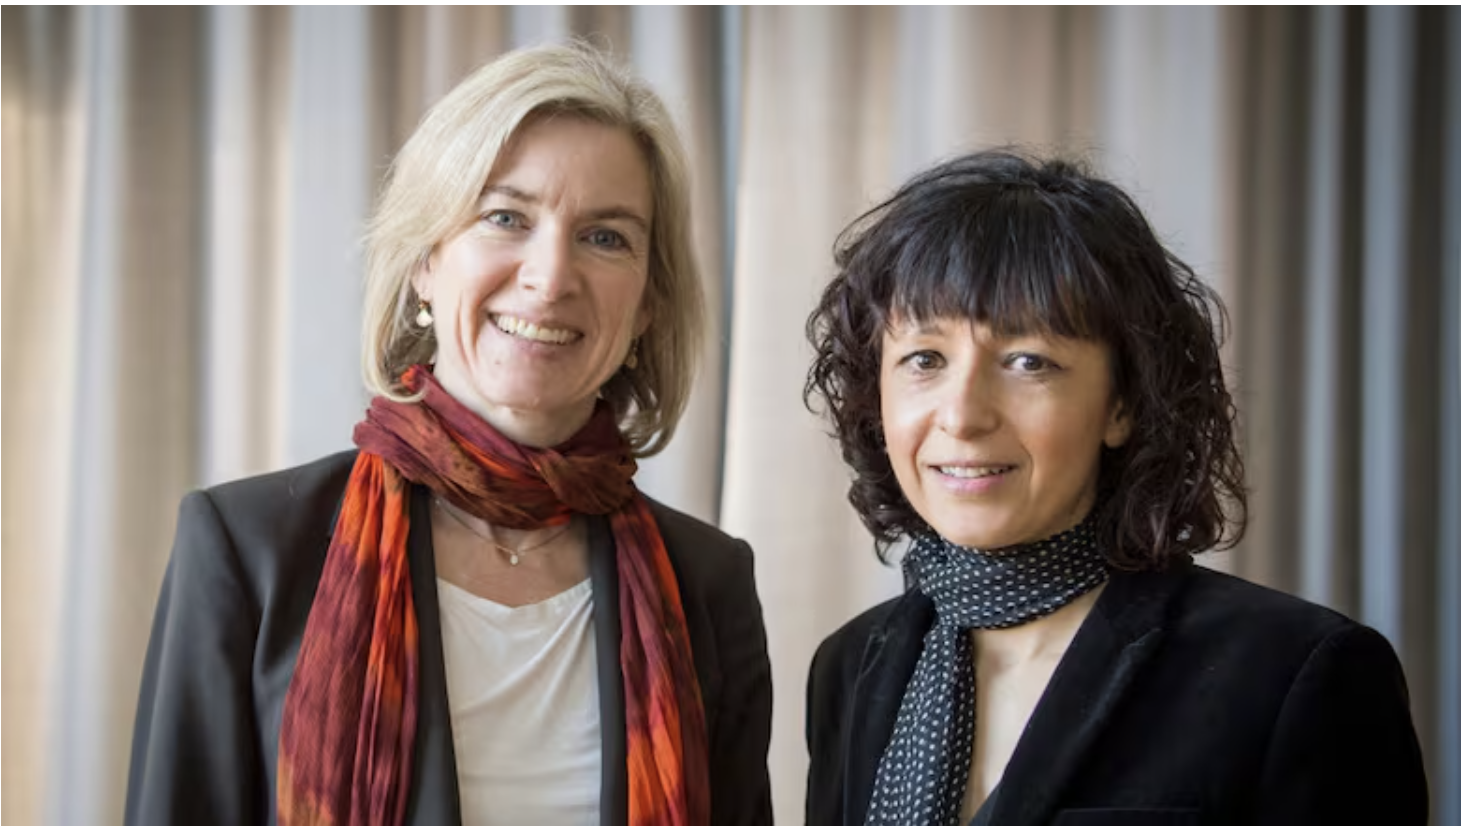
\includegraphics[keepaspectratio, width  = \textwidth]{img/nobelCRISPR_1}\\
			\Large Do you know what they won the Nobel prize for?
\end{frame}





\begin{frame}
	\frametitle{Major Milestones in Plant Breeding}
	\centering	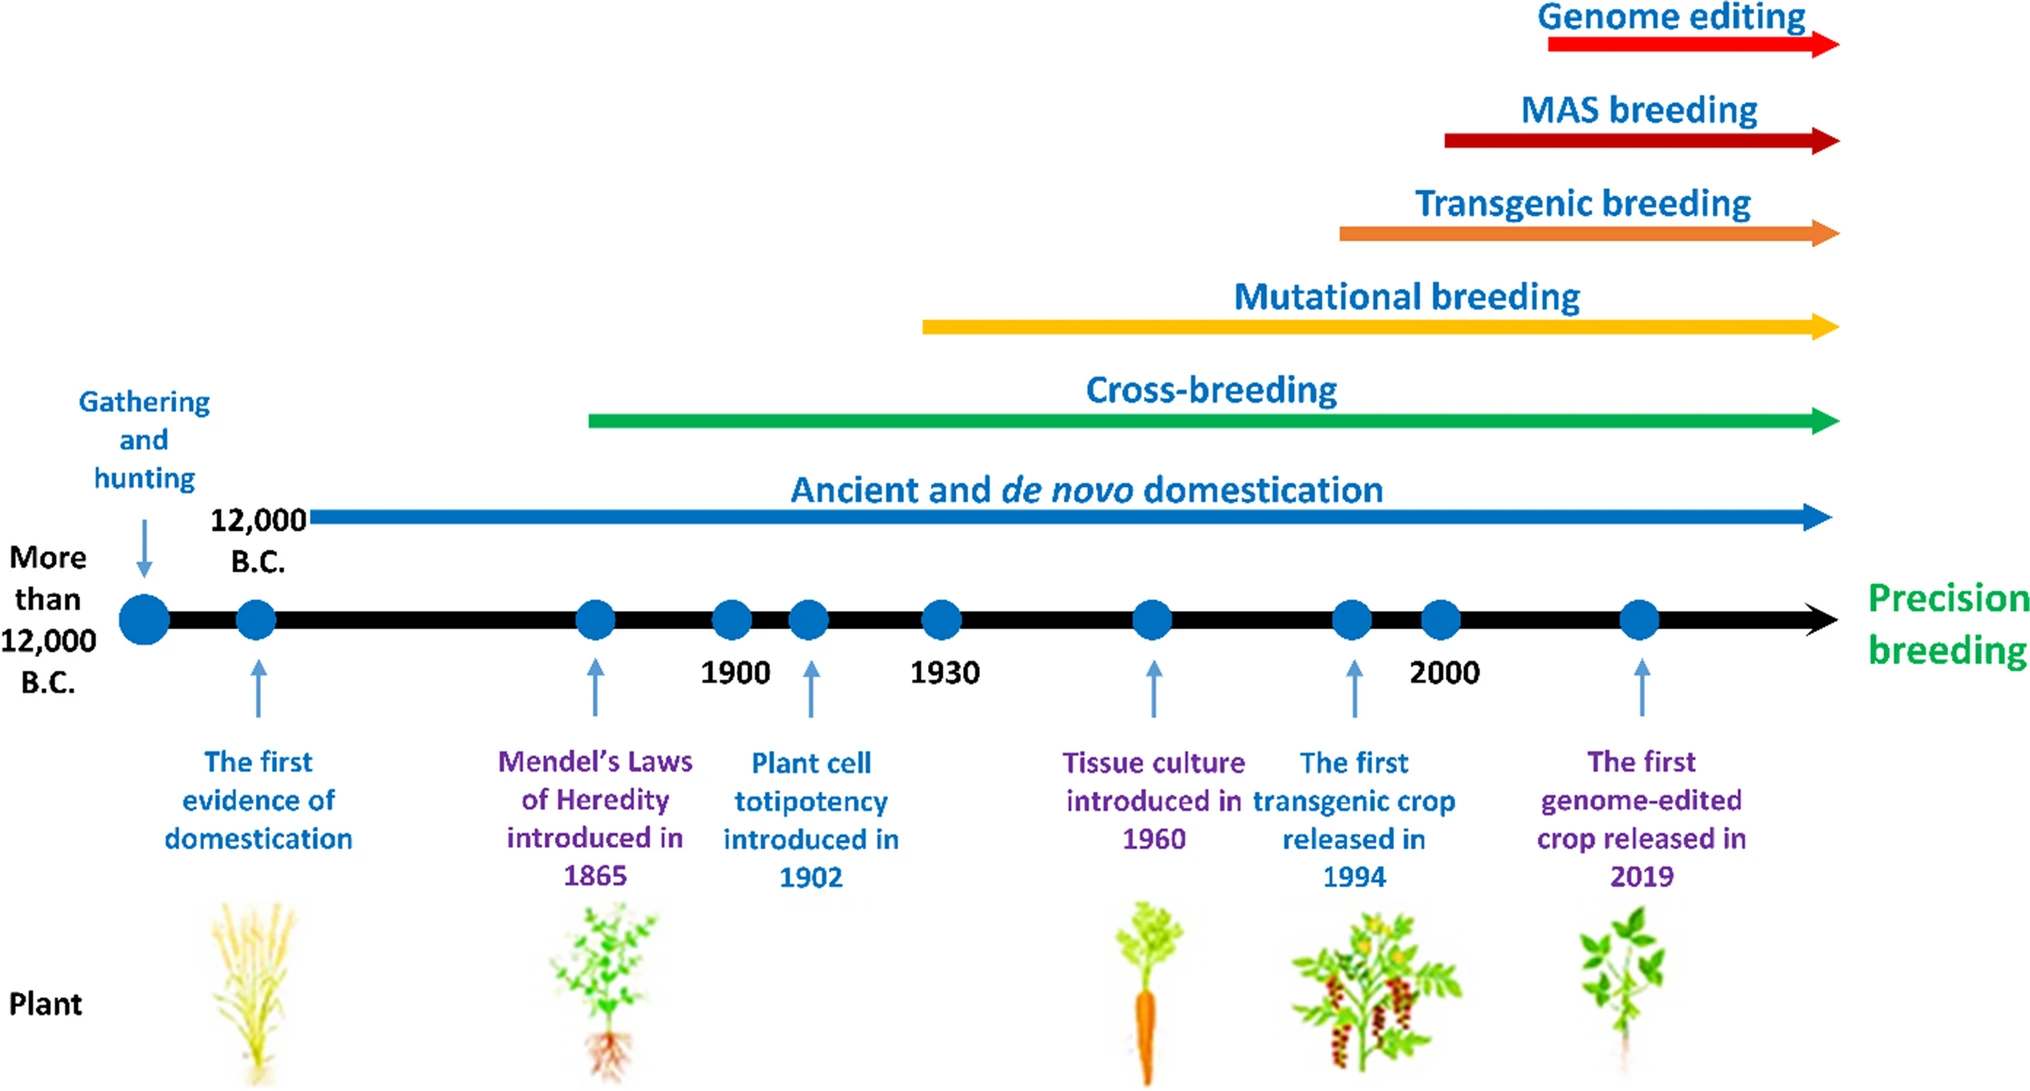
\includegraphics[keepaspectratio, width  = 0.9\textwidth]{img/timeLine}
	
	
	\begin{columns}
		\begin{column}{0.5\textwidth}
			\begin{itemize}
				\item[\textbf{1}] \st{Domestication/traditional breeding}
				\item[\textbf{2}] \st{Genetics-informed breeding}
				\item[\textbf{3}] \st{Mutational breeding}
			\end{itemize}
		\end{column}
		\begin{column}{0.5\textwidth}
			\begin{itemize}
				\item[\textbf{4}] \st{Transgenic breeding}
				\item[\textbf{5}] \st{Genomic selection} (next lecture)
				\item[\textbf{6}] Genome editing
			\end{itemize}
		\end{column}
	\end{columns}
	
	\blfootnote{Figure 1 from Van Vu et al. 2022 \textit{Planta}}
	
	
	
\end{frame}


\begin{frame}
	\frametitle{Genome Editing}
	
	\begin{itemize}
		\item[--] Genome editing is a type of genetic engineering using ``molecular scissors"
		\item[--] These ``scissors" create site-specific double-strand breaks \textbf{at desired locations }in the genome. 
		\item[--] The induced double-strand breaks are repaired with errors, resulting in targeted mutations ('edits').
		
	\end{itemize} \pause
	\vspace{10pt}
	
	\large Limitations of GM not shared by genome editing
	%%%
	\normalsize 
	\begin{columns}
		\begin{column}{0.5\textwidth}
			\begin{itemize}
				\item[--] \st{The insertion of a new gene may not occur} 
				\item[--] \st{No control on targeting DNA locations}
				
			\end{itemize}
		\end{column}
		\begin{column}{0.5\textwidth}
			\begin{itemize}
				\item[--] \st{One gene at a time}
				\item[--] \st{Expensive and slow}
				\item[--] Under strict regulation
			\end{itemize}
			
		\end{column}
	\end{columns}
\end{frame}




\begin{frame}
	\frametitle{CRISPR-Cas9}
	
	Genome editing is typically achieved using the CRISPR/Cas system\\
	\centering{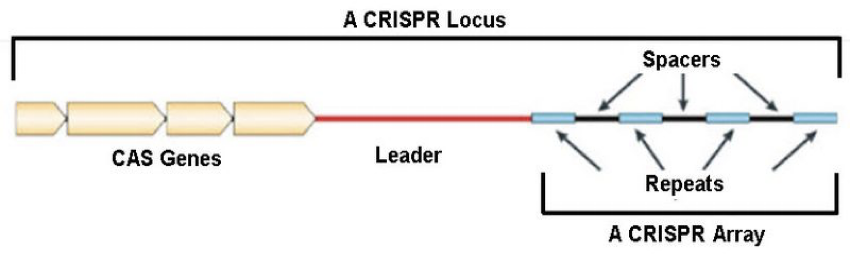
\includegraphics[keepaspectratio, width  = 0.7\textwidth]{img/CRISPR_locus}}\\
	
	\textbf{C}lustered \textbf{R}egularly \textbf{I}nterspaced \textbf{S}hort \textbf{P}alindromic \textbf{R}epeats
	\flushleft
	The CRISPR/Cas system is a bacterial immune system that confers resistance to foreign genetic elements and provides a form of acquired immunity
	
	
	\blfootnote{Here's a simple video overview: \url{https://youtu.be/6tw_JVz_IEc?si=_H2TrKqrd5rSOpEL}}
\end{frame}



\begin{frame}
	\frametitle{CRISPR-Cas9}
	
	Genome editing is typically achieved using the CRISPR/Cas system\\
	\centering{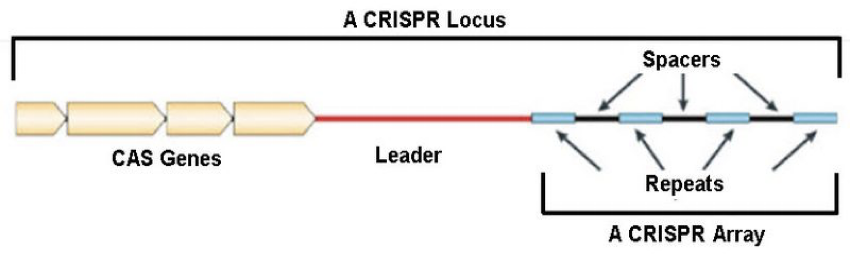
\includegraphics[keepaspectratio, width  = 0.7\textwidth]{img/CRISPR_locus}}\\
	
	\textbf{C}lustered \textbf{R}egularly \textbf{I}nterspaced \textbf{S}hort \textbf{P}alindromic \textbf{R}epeats
	\flushleft

	A CRISPR locus: \\
	
	\begin{itemize}
		\item[--] Encodes the Cas9 protein (the ``scissors")
		\item[--] Transcribes a guide RNA to find the target
	\end{itemize} 
			
The two components form a complex to find and destroy the target DNA
	
	
	\blfootnote{Here's a simple video overview: \url{https://youtu.be/6tw_JVz_IEc?si=_H2TrKqrd5rSOpEL}}
\end{frame}





\begin{frame}
	\frametitle{CRISPR and Gene Editing}
	
	
	\begin{columns}
		\begin{column}{0.5\textwidth}
			\begin{itemize}
				\item[--] CRISPR/Cas9 induces a double strand break at a specific DNA sequence
				\item[--] Adding a synthetic ``guide" can direct the system to make arbitrary cuts
				\item[--] Add a custom exogenous DNA template for DNA repair to incorate into the host's genome
			\end{itemize}
		\end{column}
		\begin{column}{0.5\textwidth}
			\centering{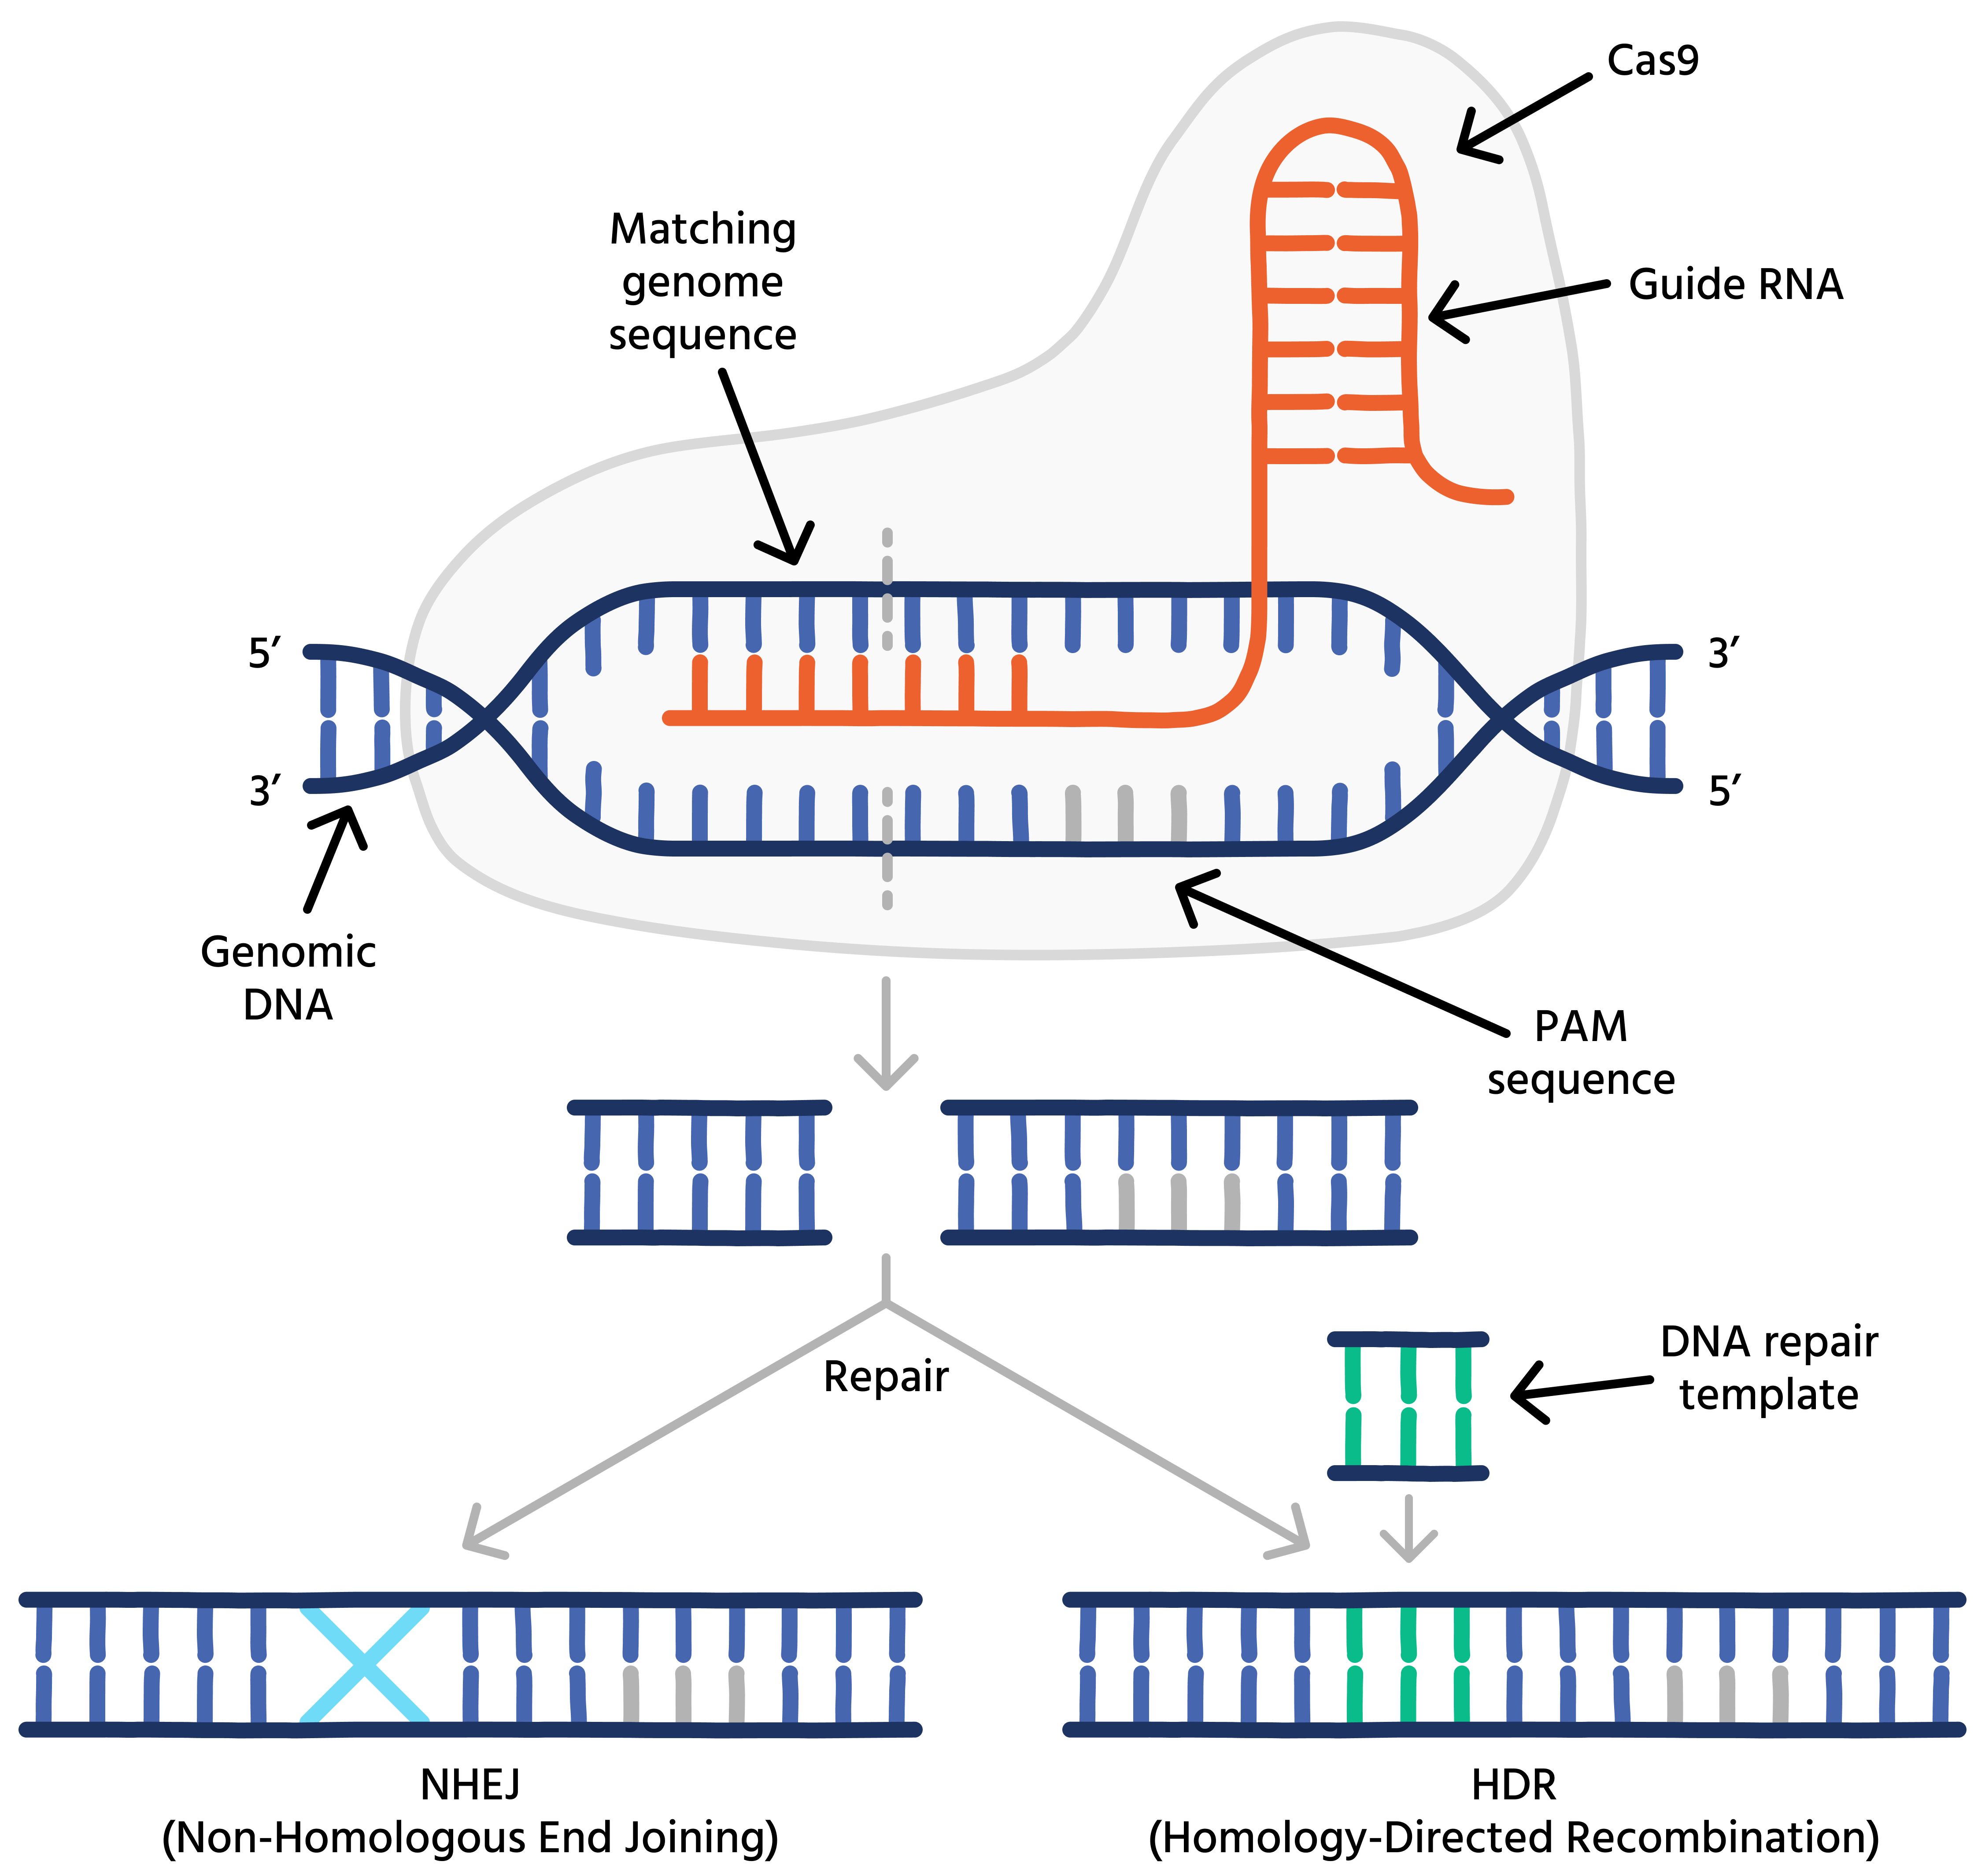
\includegraphics[keepaspectratio, width  = \textwidth]{img/CRISPR-Cas9_mechanism	}}\\
		\end{column}
	\end{columns}
	\vspace{10pt}
	
	
	
	By \textit{editing} DNA rather than inserting it, a wider range of changes are made possible
	\blfootnote{}
\end{frame}

\begin{frame}
	\frametitle{Unintended Side Effects}
	
	\begin{columns}
		\begin{column}{0.5\textwidth}
Genome editing with CRISPR/Cas9 can cause DNA deletions and rearrangements near the target site on the genome\\
\vspace{15pt}
A problem for clinical applications, maybe less so for in the context of plant breeding

		\end{column}
		\begin{column}{0.5\textwidth}
				\centering{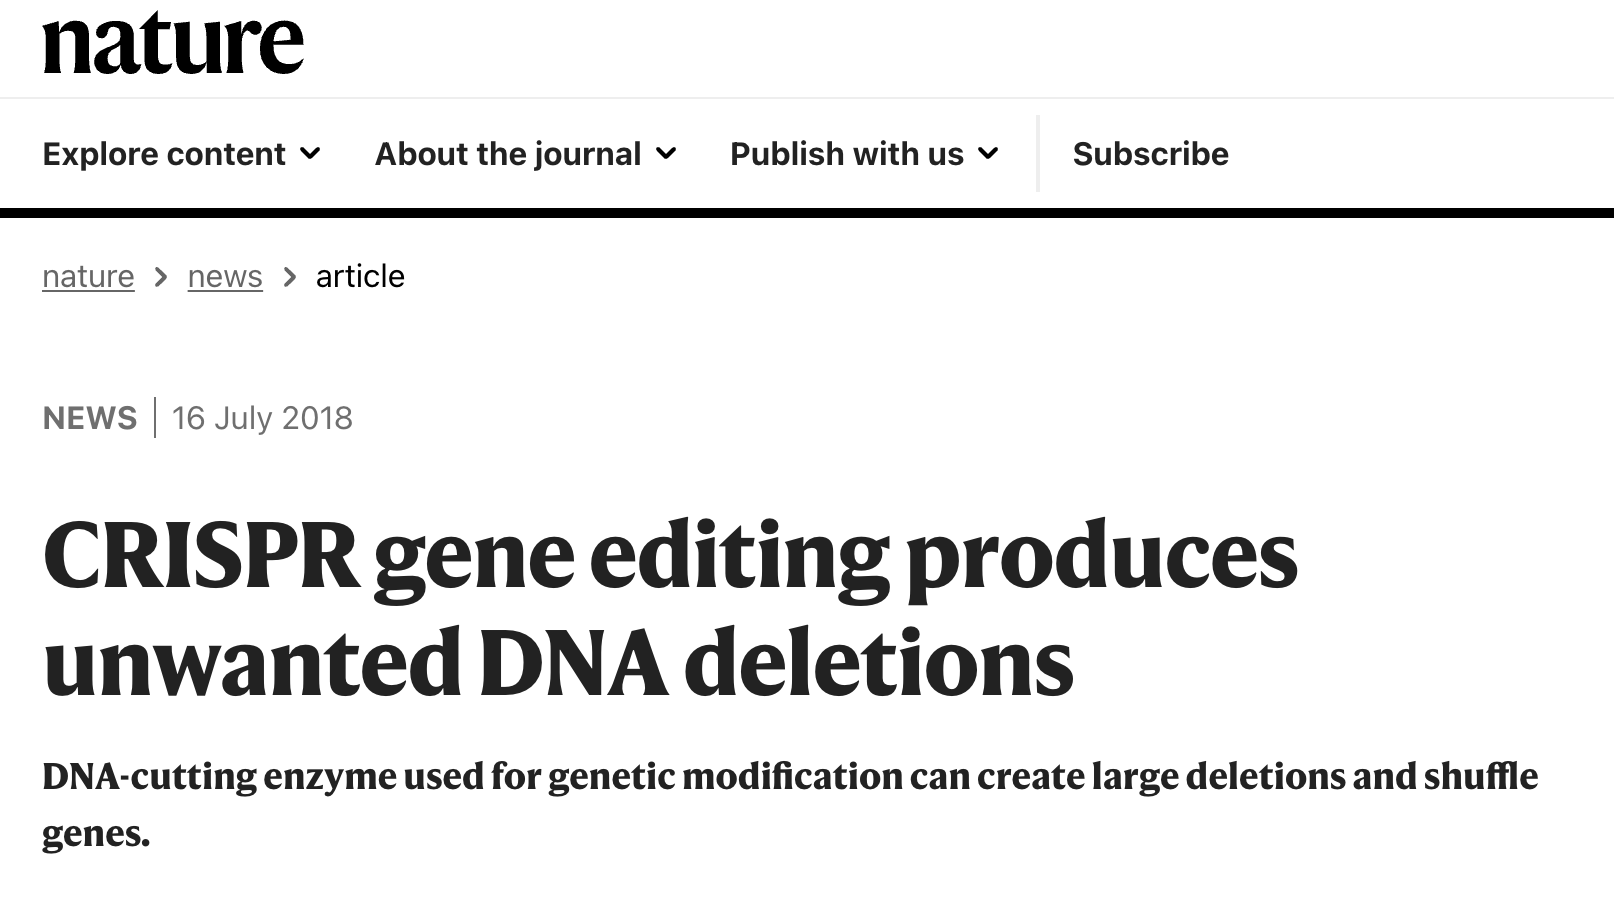
\includegraphics[keepaspectratio, width  = \textwidth]{img/CRISPR_sideEffects}}\\
\end{column}
	\end{columns}
	\blfootnote{Individuals with deleterious side effects from CRISPR could simply be removed from circulation}
\end{frame}



\begin{frame}
	
	\scriptsize{Put ethical, ecological and economic concerns aside for the moment...}
	
	\Huge{What are some ways that genome editing be used in forest trees?}
	
\end{frame}


\begin{frame}
	\frametitle{Lignin Removal}
		\centering{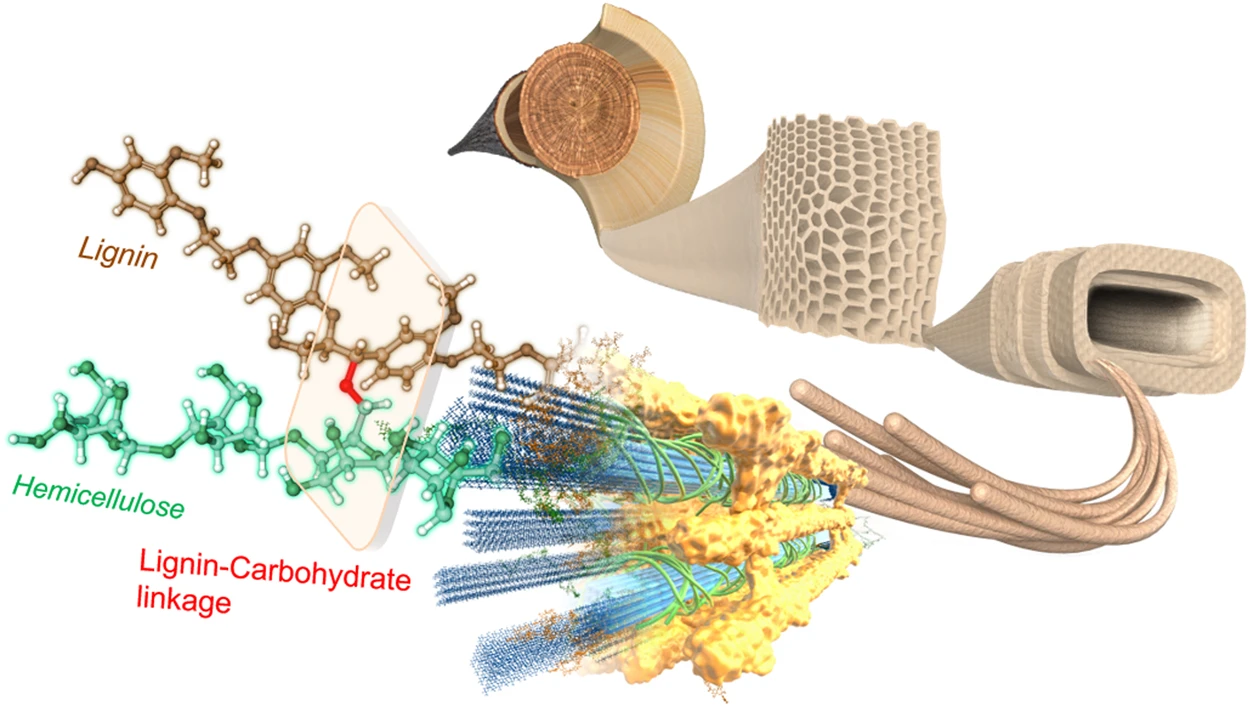
\includegraphics[keepaspectratio, width  = 0.7\textwidth]{img/ligninInWood}}\\	
\flushleft
\scriptsize
\begin{itemize}
				\item[]	Lignin is one of the most abundant polymers on earth	
			\item[] Removal of lignin from pulp is a key part of paper manufacture
			\item[] High density engineered wood can be made from wood that has been treated for reduced lignin 
			\item[] The process of delignification consumes energy and generates toxic byproducs
			\end{itemize}
\blfootnote{Nishimura et al. 2018 \textit{Sci. Reports}	}
\end{frame}


\begin{frame}
	\frametitle{Lignin Biosynthesis}
					\centering{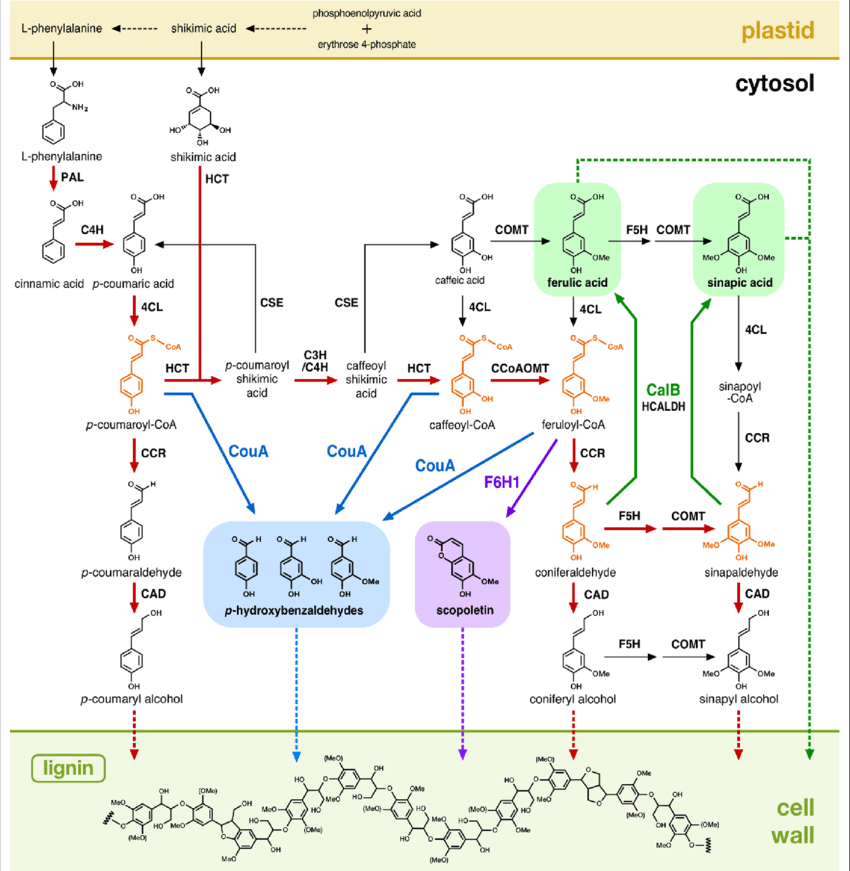
\includegraphics[keepaspectratio, width  = 0.7\textwidth]{img/ligninBiosynthesis}}\\


\end{frame}





\begin{frame}
	\frametitle{Genome Editing to Reduce Lignin Content}
	
						\centering{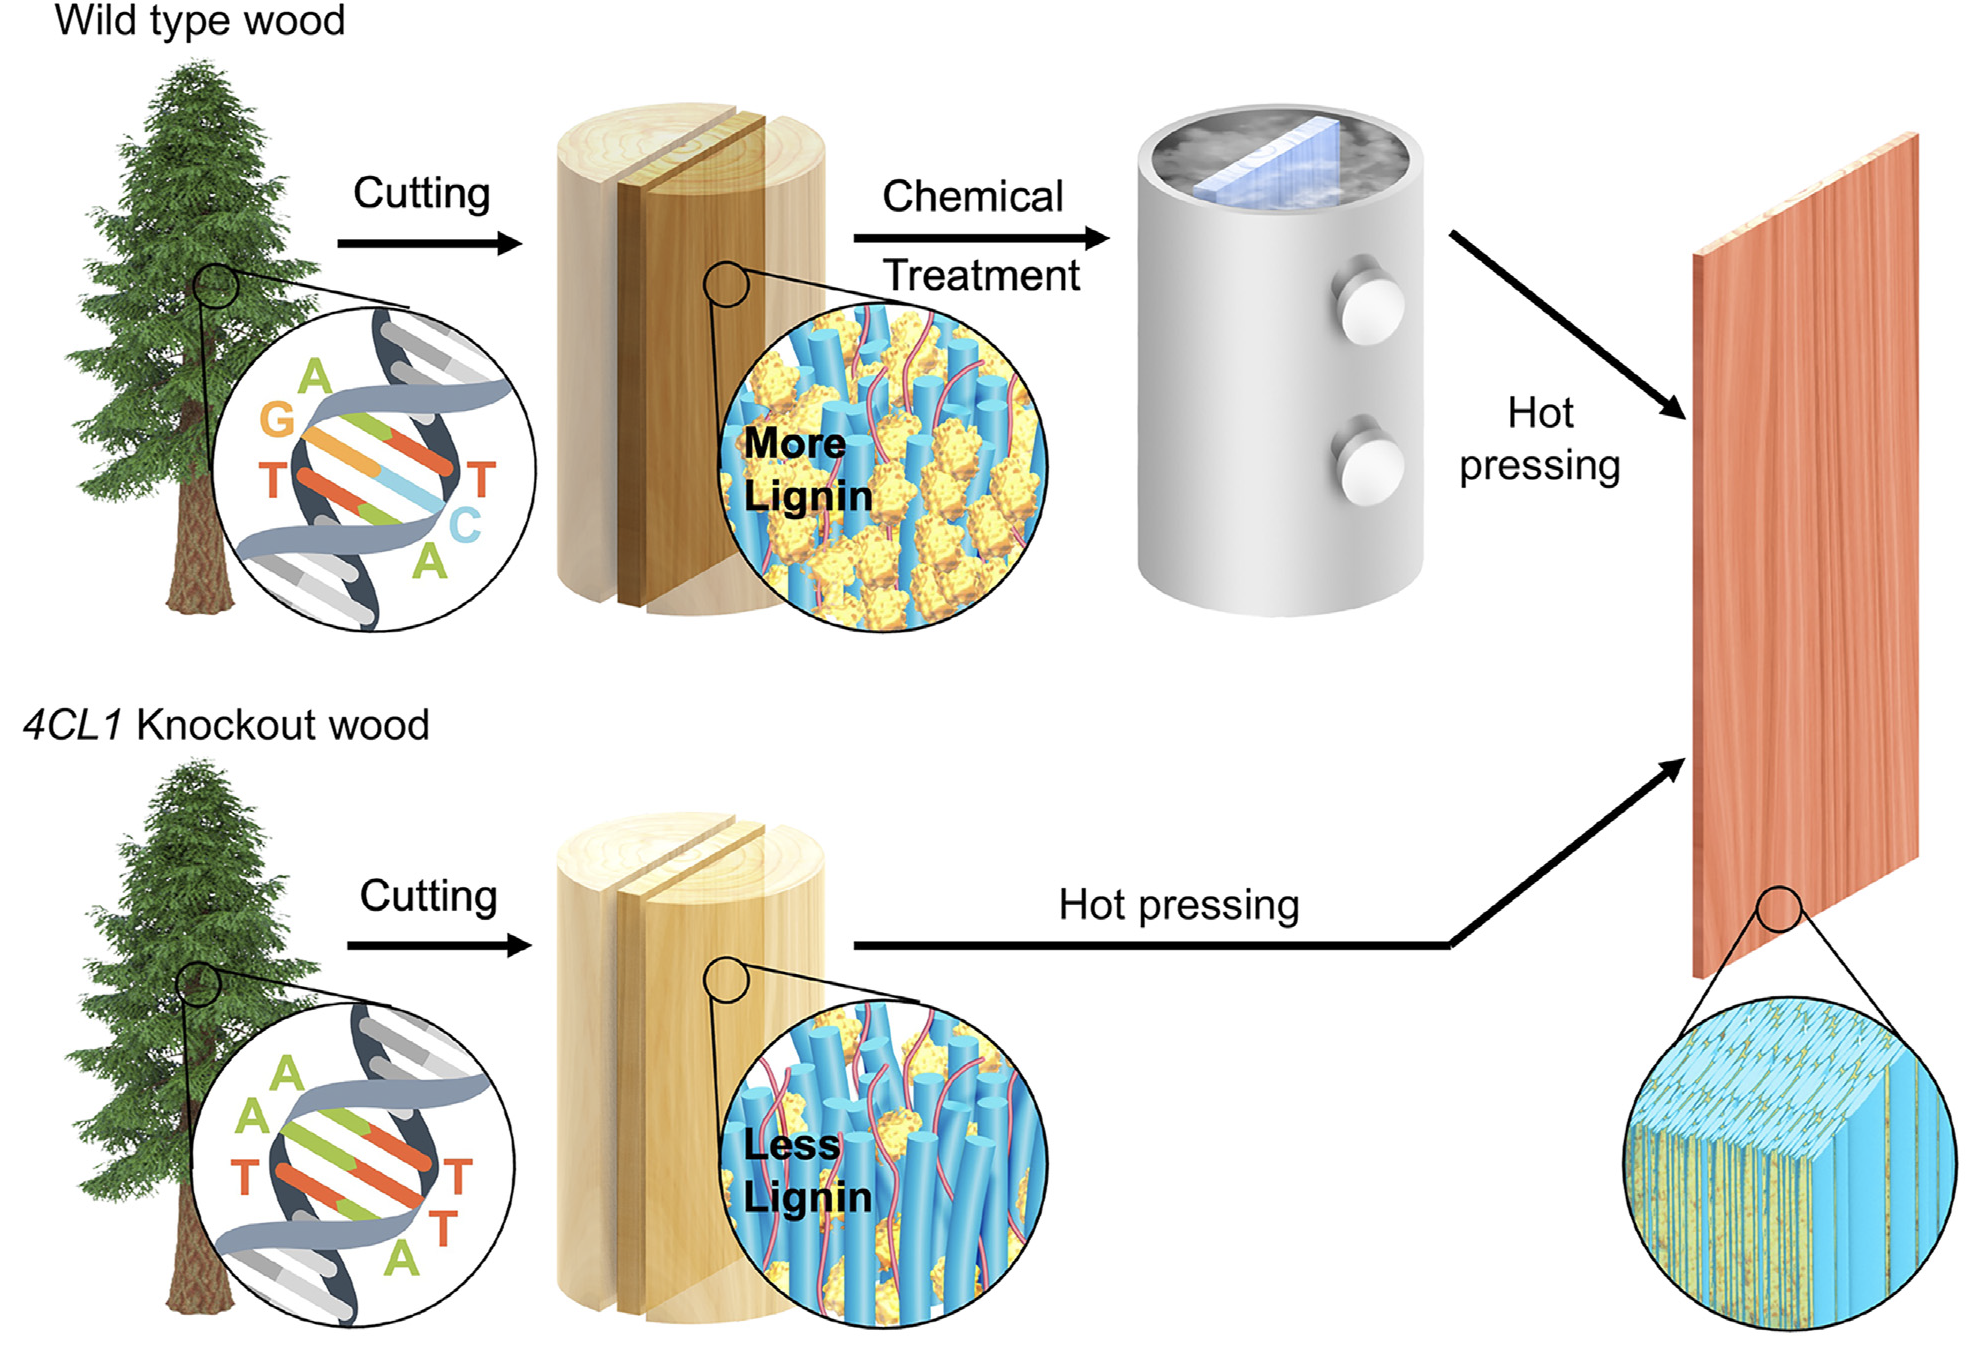
\includegraphics[keepaspectratio, width  = 0.8\textwidth]{img/4CL1_knockout}}\\
						\blfootnote{Liu et al 2024 Matter}
\end{frame}



\begin{frame}
	\frametitle{Genome Editing to Reduce Lignin Content}
	
	
	\begin{columns}
		\begin{column}{0.5\textwidth}
			\centering{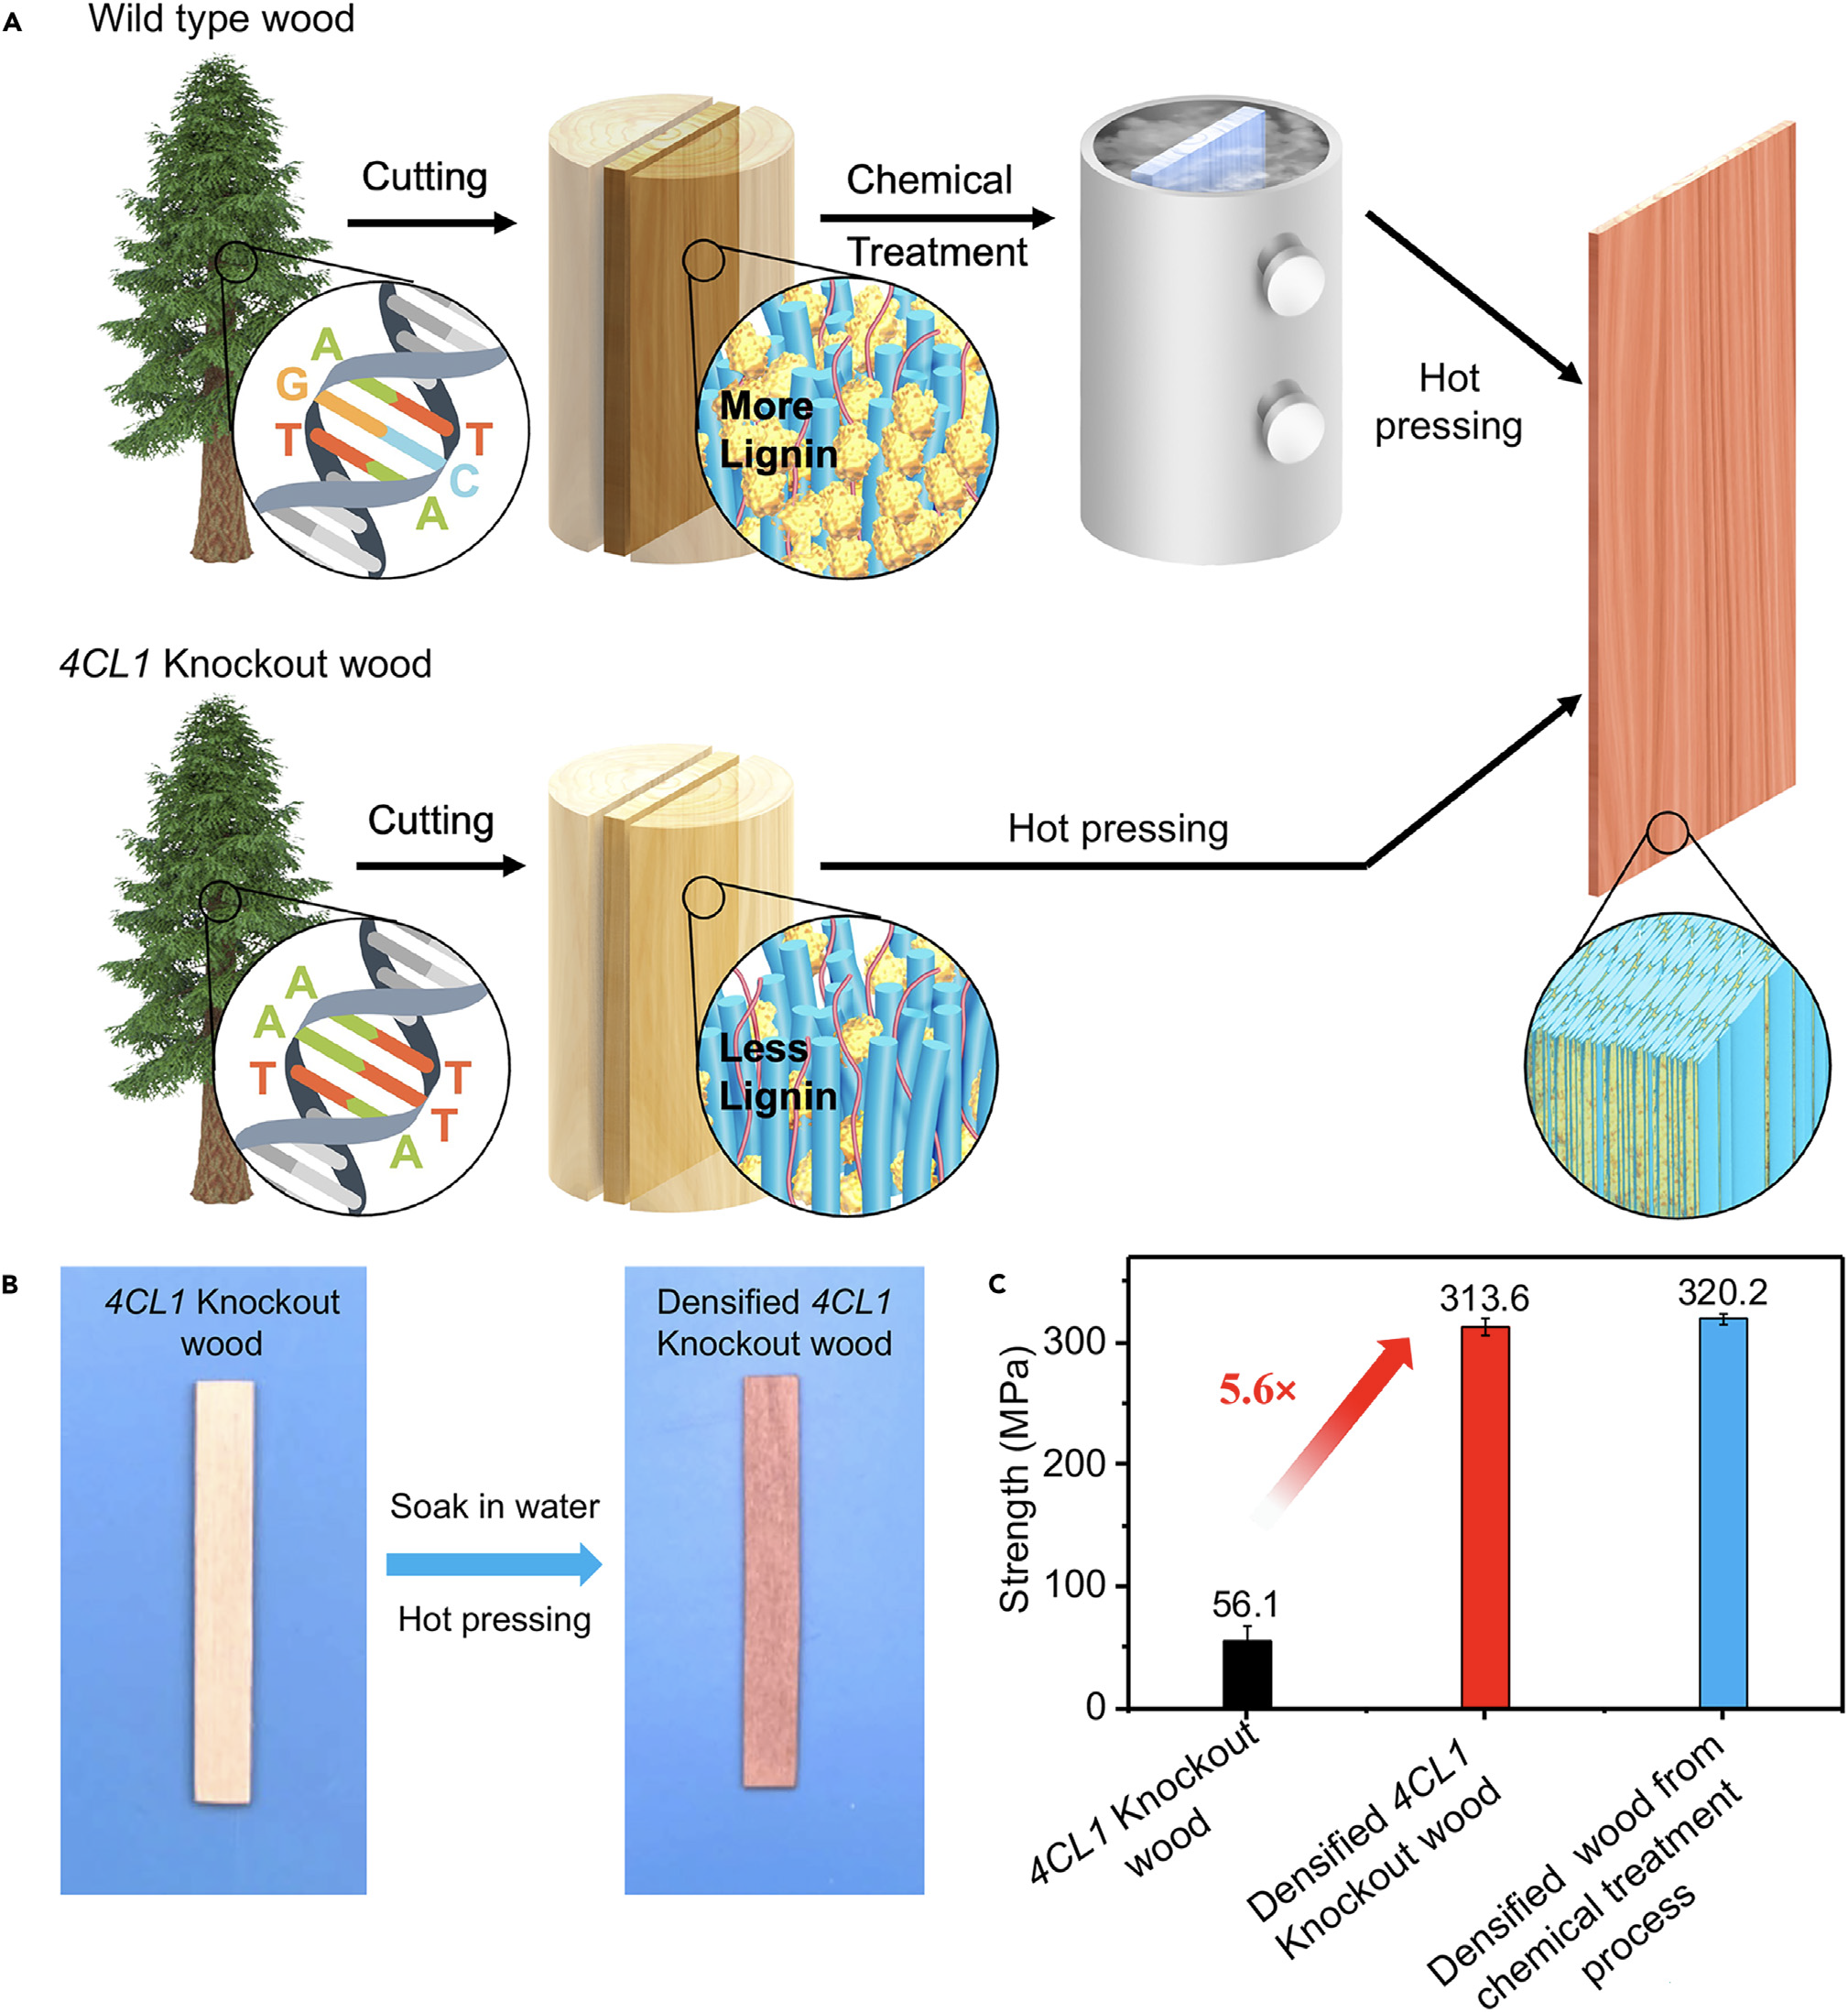
\includegraphics[keepaspectratio, width  = \textwidth]{img/4CL1_knockoutTrees_full}}
		\end{column}
		\begin{column}{0.5\textwidth}
			\centering{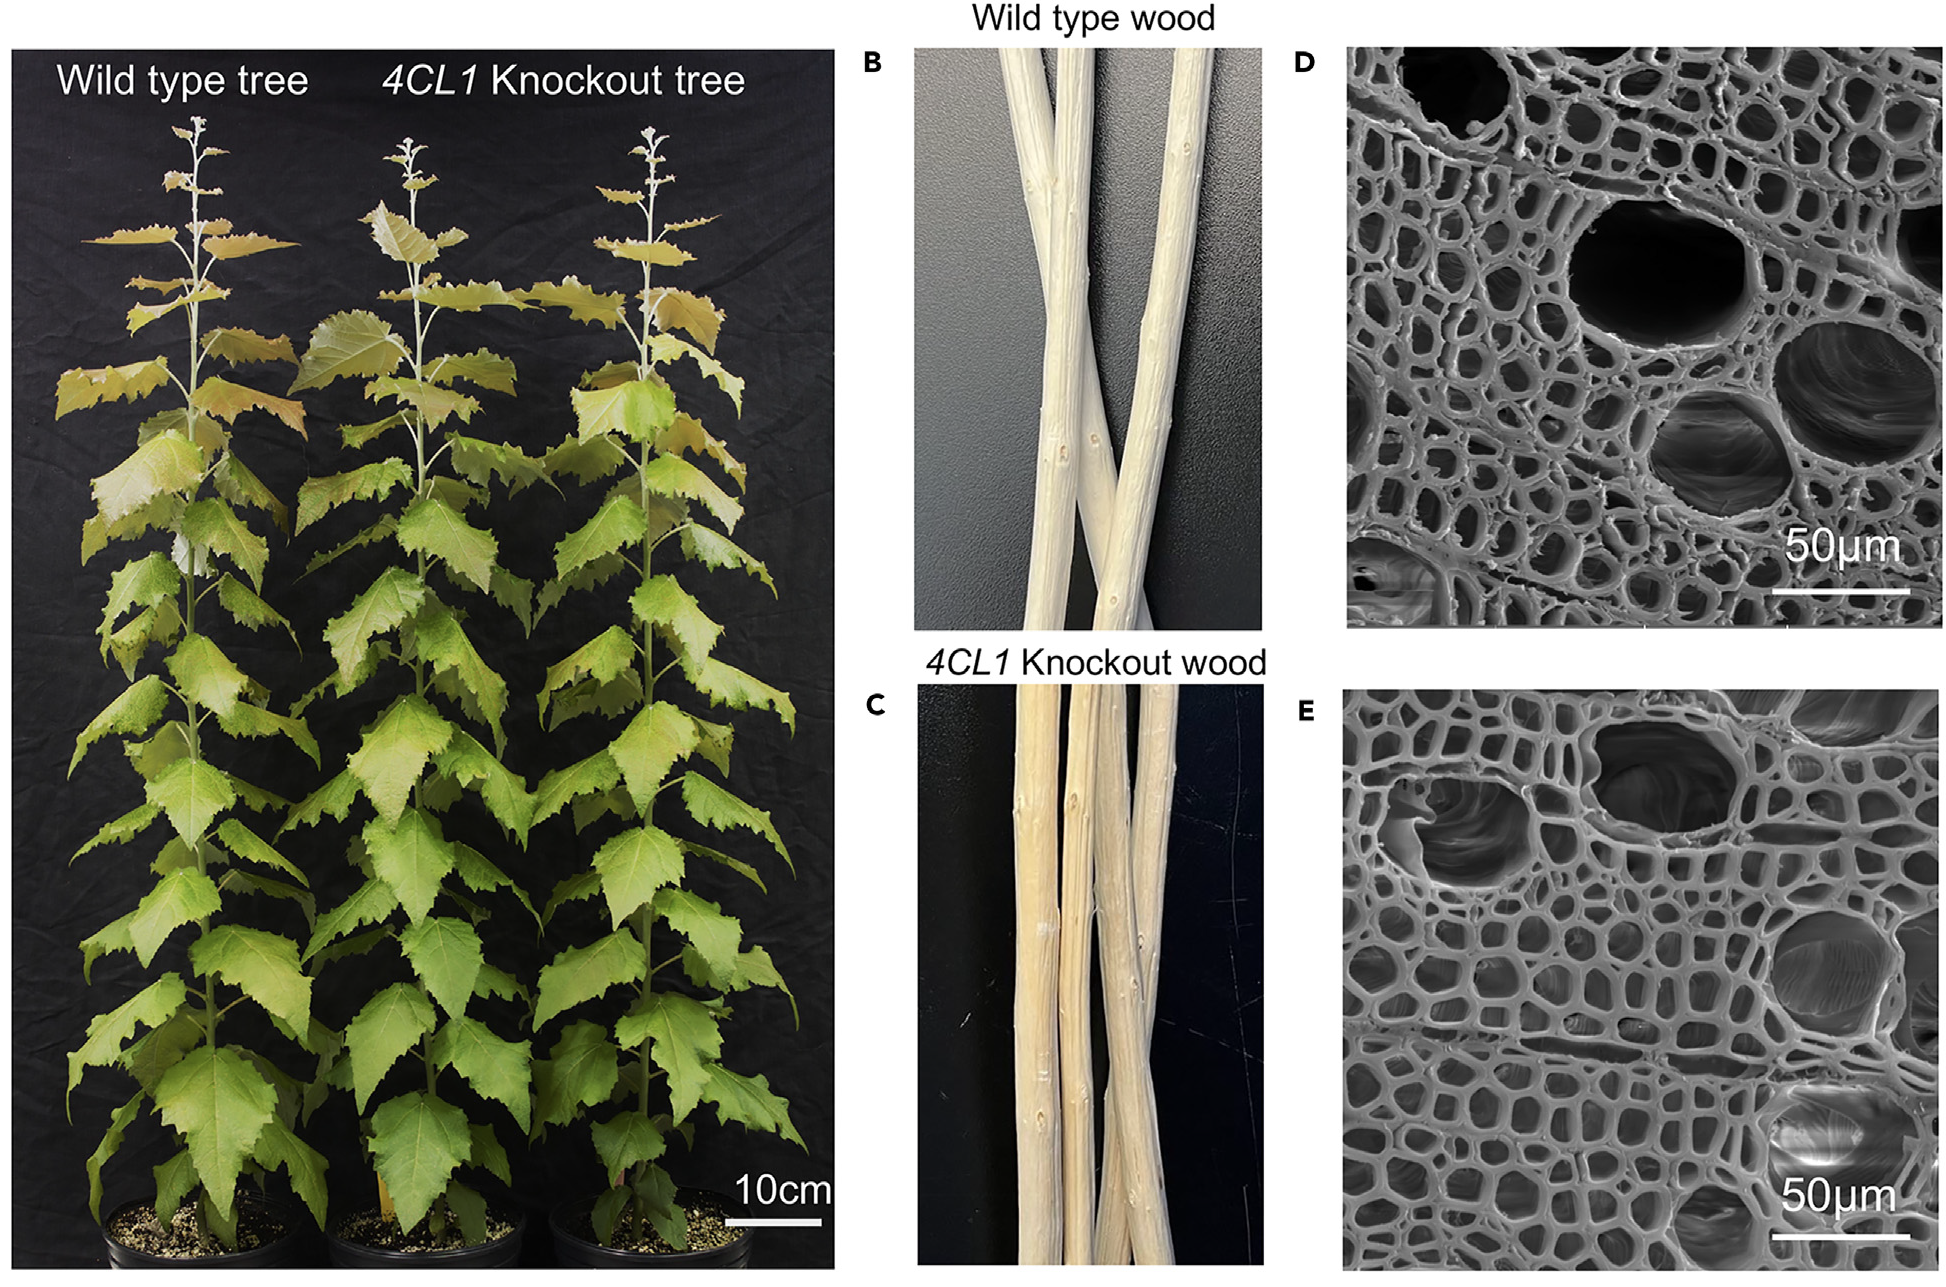
\includegraphics[keepaspectratio, width  = \textwidth]{img/4CL1_knockoutTrees}}
		\end{column}
	\end{columns}
	
	
	
	
						\blfootnote{Figures 1 and 2 (modified) from Liu et al 2024 Matter}
						\end{frame}



\begin{frame}
	
	\frametitle{Learning Outcomes}
	
	Association genetics
	
	Statistical issues in association genetics:
	\begin{itemize}
		\item[--]   Population structure can lead to false positives
		\item[--]	Multiple comparisons makes tests more stringent
		\item[--]   Works well for large effect loci, not so much for small effects
		\item[--]	Effect sizes may be upwardly biased (i.e. Beavis effect)
	\end{itemize}

\end{frame}
\begin{frame}
	\frametitle{A Question to Think About...}
	
	
	
\end{frame}

\begin{frame}
\scriptsize
		\begin{tabular}{c|c|c|c|c}
			Traditional Breeding &Genetics-informed Breeding & Mutational Breeding & Transgenic Breeding & Genome Editing \\
				
			\end{tabular}
\end{frame}

\end{document}


%%%
\begin{columns}
	\begin{column}{0.5\textwidth}
	\end{column}
	\begin{column}{0.5\textwidth}
	\end{column}
\end{columns}



